\documentclass[]{book}
\usepackage{lmodern}
\usepackage{amssymb,amsmath}
\usepackage{ifxetex,ifluatex}
\usepackage{fixltx2e} % provides \textsubscript
\ifnum 0\ifxetex 1\fi\ifluatex 1\fi=0 % if pdftex
  \usepackage[T1]{fontenc}
  \usepackage[utf8]{inputenc}
\else % if luatex or xelatex
  \ifxetex
    \usepackage{mathspec}
  \else
    \usepackage{fontspec}
  \fi
  \defaultfontfeatures{Ligatures=TeX,Scale=MatchLowercase}
\fi
% use upquote if available, for straight quotes in verbatim environments
\IfFileExists{upquote.sty}{\usepackage{upquote}}{}
% use microtype if available
\IfFileExists{microtype.sty}{%
\usepackage{microtype}
\UseMicrotypeSet[protrusion]{basicmath} % disable protrusion for tt fonts
}{}
\usepackage[margin=1in]{geometry}
\usepackage{hyperref}
\hypersetup{unicode=true,
            pdftitle={Applied Missing data analysis with SPSS and R(Studio)},
            pdfauthor={Martijn Heymans and Iris Eekhout},
            pdfborder={0 0 0},
            breaklinks=true}
\urlstyle{same}  % don't use monospace font for urls
\usepackage{natbib}
\bibliographystyle{apalike}
\usepackage{color}
\usepackage{fancyvrb}
\newcommand{\VerbBar}{|}
\newcommand{\VERB}{\Verb[commandchars=\\\{\}]}
\DefineVerbatimEnvironment{Highlighting}{Verbatim}{commandchars=\\\{\}}
% Add ',fontsize=\small' for more characters per line
\usepackage{framed}
\definecolor{shadecolor}{RGB}{248,248,248}
\newenvironment{Shaded}{\begin{snugshade}}{\end{snugshade}}
\newcommand{\KeywordTok}[1]{\textcolor[rgb]{0.13,0.29,0.53}{\textbf{#1}}}
\newcommand{\DataTypeTok}[1]{\textcolor[rgb]{0.13,0.29,0.53}{#1}}
\newcommand{\DecValTok}[1]{\textcolor[rgb]{0.00,0.00,0.81}{#1}}
\newcommand{\BaseNTok}[1]{\textcolor[rgb]{0.00,0.00,0.81}{#1}}
\newcommand{\FloatTok}[1]{\textcolor[rgb]{0.00,0.00,0.81}{#1}}
\newcommand{\ConstantTok}[1]{\textcolor[rgb]{0.00,0.00,0.00}{#1}}
\newcommand{\CharTok}[1]{\textcolor[rgb]{0.31,0.60,0.02}{#1}}
\newcommand{\SpecialCharTok}[1]{\textcolor[rgb]{0.00,0.00,0.00}{#1}}
\newcommand{\StringTok}[1]{\textcolor[rgb]{0.31,0.60,0.02}{#1}}
\newcommand{\VerbatimStringTok}[1]{\textcolor[rgb]{0.31,0.60,0.02}{#1}}
\newcommand{\SpecialStringTok}[1]{\textcolor[rgb]{0.31,0.60,0.02}{#1}}
\newcommand{\ImportTok}[1]{#1}
\newcommand{\CommentTok}[1]{\textcolor[rgb]{0.56,0.35,0.01}{\textit{#1}}}
\newcommand{\DocumentationTok}[1]{\textcolor[rgb]{0.56,0.35,0.01}{\textbf{\textit{#1}}}}
\newcommand{\AnnotationTok}[1]{\textcolor[rgb]{0.56,0.35,0.01}{\textbf{\textit{#1}}}}
\newcommand{\CommentVarTok}[1]{\textcolor[rgb]{0.56,0.35,0.01}{\textbf{\textit{#1}}}}
\newcommand{\OtherTok}[1]{\textcolor[rgb]{0.56,0.35,0.01}{#1}}
\newcommand{\FunctionTok}[1]{\textcolor[rgb]{0.00,0.00,0.00}{#1}}
\newcommand{\VariableTok}[1]{\textcolor[rgb]{0.00,0.00,0.00}{#1}}
\newcommand{\ControlFlowTok}[1]{\textcolor[rgb]{0.13,0.29,0.53}{\textbf{#1}}}
\newcommand{\OperatorTok}[1]{\textcolor[rgb]{0.81,0.36,0.00}{\textbf{#1}}}
\newcommand{\BuiltInTok}[1]{#1}
\newcommand{\ExtensionTok}[1]{#1}
\newcommand{\PreprocessorTok}[1]{\textcolor[rgb]{0.56,0.35,0.01}{\textit{#1}}}
\newcommand{\AttributeTok}[1]{\textcolor[rgb]{0.77,0.63,0.00}{#1}}
\newcommand{\RegionMarkerTok}[1]{#1}
\newcommand{\InformationTok}[1]{\textcolor[rgb]{0.56,0.35,0.01}{\textbf{\textit{#1}}}}
\newcommand{\WarningTok}[1]{\textcolor[rgb]{0.56,0.35,0.01}{\textbf{\textit{#1}}}}
\newcommand{\AlertTok}[1]{\textcolor[rgb]{0.94,0.16,0.16}{#1}}
\newcommand{\ErrorTok}[1]{\textcolor[rgb]{0.64,0.00,0.00}{\textbf{#1}}}
\newcommand{\NormalTok}[1]{#1}
\usepackage{longtable,booktabs}
\usepackage{graphicx,grffile}
\makeatletter
\def\maxwidth{\ifdim\Gin@nat@width>\linewidth\linewidth\else\Gin@nat@width\fi}
\def\maxheight{\ifdim\Gin@nat@height>\textheight\textheight\else\Gin@nat@height\fi}
\makeatother
% Scale images if necessary, so that they will not overflow the page
% margins by default, and it is still possible to overwrite the defaults
% using explicit options in \includegraphics[width, height, ...]{}
\setkeys{Gin}{width=\maxwidth,height=\maxheight,keepaspectratio}
\IfFileExists{parskip.sty}{%
\usepackage{parskip}
}{% else
\setlength{\parindent}{0pt}
\setlength{\parskip}{6pt plus 2pt minus 1pt}
}
\setlength{\emergencystretch}{3em}  % prevent overfull lines
\providecommand{\tightlist}{%
  \setlength{\itemsep}{0pt}\setlength{\parskip}{0pt}}
\setcounter{secnumdepth}{5}
% Redefines (sub)paragraphs to behave more like sections
\ifx\paragraph\undefined\else
\let\oldparagraph\paragraph
\renewcommand{\paragraph}[1]{\oldparagraph{#1}\mbox{}}
\fi
\ifx\subparagraph\undefined\else
\let\oldsubparagraph\subparagraph
\renewcommand{\subparagraph}[1]{\oldsubparagraph{#1}\mbox{}}
\fi

%%% Use protect on footnotes to avoid problems with footnotes in titles
\let\rmarkdownfootnote\footnote%
\def\footnote{\protect\rmarkdownfootnote}

%%% Change title format to be more compact
\usepackage{titling}

% Create subtitle command for use in maketitle
\newcommand{\subtitle}[1]{
  \posttitle{
    \begin{center}\large#1\end{center}
    }
}

\setlength{\droptitle}{-2em}

  \title{Applied Missing data analysis with SPSS and R(Studio)}
    \pretitle{\vspace{\droptitle}\centering\huge}
  \posttitle{\par}
    \author{Martijn Heymans and Iris Eekhout}
    \preauthor{\centering\large\emph}
  \postauthor{\par}
      \predate{\centering\large\emph}
  \postdate{\par}
    \date{2018-09-04}

\usepackage{booktabs}

\usepackage{amsthm}
\newtheorem{theorem}{Theorem}[chapter]
\newtheorem{lemma}{Lemma}[chapter]
\theoremstyle{definition}
\newtheorem{definition}{Definition}[chapter]
\newtheorem{corollary}{Corollary}[chapter]
\newtheorem{proposition}{Proposition}[chapter]
\theoremstyle{definition}
\newtheorem{example}{Example}[chapter]
\theoremstyle{definition}
\newtheorem{exercise}{Exercise}[chapter]
\theoremstyle{remark}
\newtheorem*{remark}{Remark}
\newtheorem*{solution}{Solution}
\begin{document}
\maketitle

{
\setcounter{tocdepth}{1}
\tableofcontents
}
\chapter*{Preface}\label{preface}
\addcontentsline{toc}{chapter}{Preface}

The attention for missing data is growing and so will be the application
of methods to solve the missing data problem. From our experience,
researchers with missing data still find it difficult to reserve time to
evaluate the missing data and from that to find a reasonable solution to
handle their missing data for their main data analysis. This manual is
developed for researchers that are looking for a solution of their
missing data problem or want to learn more about missing data. The
manual is developed as a result of a missing data course that we give.
Further, we are also active in providing statistical advice in general
and more specific about missing data. Because our time to give advice is
mostly limited we wanted to give researchers a practical guide to help
them get started with their missing data problem. Leading methodologists
and statisticians and leading journals have published papers about the
problems of missing data and warned researchers to take missing data
seriously (Sterne et al., BMJ 2009, Little et al. NEJM 2012, Peng et al.
2015, JAMA). Hopefully this manual will help researchers to find the
best solution for their missing data problem. We hope you will enjoy
this manual and that you learn from it, at least to take missing data
seriously and that you will use recommended methods to solve your
missing data problem.

\section{The goal of this Manual}\label{the-goal-of-this-manual}

In this manual the software packages SPSS and R play a central role. The
combination of these two software packages may seem a coincidence, but
it is not. For a long time, SPSS was the most popular software package
worldwide to do statistical data analysis. Currently, R is growing in
popularity fast and will probably become one of the most popular
Software packages to do data analysis. Also for applied researchers.
Both SPSS and R have their advantages and disadvantages. An advantage of
SPSS is that it is a user-friendly software package compared to R and
works with windows where you can for example drag your variables to.
Subsequently, you can click the OK button and the statistical analysis
procedure you prespecified gives you the output results. A disadvantage
of SPSS may be that you are overloaded with statistical output that may
not all needed to answer your research question. Compared to SPSS you
could say that R is a more user-unfriendly software package where you
need to use R code to activate statistical procedures and to get
statistical results. R output will show more specific results, without
extra information. Furthermore, R works much faster when it comes to
running statistical procedures by using 1 or 2 lines of R code, compared
to visiting a couple of windows in SPSS to activate the same statistical
test. There is one other advantage of R and that is, that it is open
source. This makes it possible for applied researchers to follow the
calculations of complex procedures as the estimation of missing values
closely along the line. You could say that R brings you to the heart of
the matter. With R it is possible to turn complex data analysis
functions and formula´s into computer code that can be used by everybody
and vice versa. Because it is open source, you are able to read the code
that is used for the analysis and to relate that code or pieces of code
to the statistical output. This makes it possible to evaluate step by
step the code and thus the statistical procedures and relate them to the
subsequent results. You can copy specific parts of code from functions
that others have written and evaluate what happens. This is one of the
major advantages of R if you compare it to the closed source statistical
package SPSS. R brings you a big learning environment when it comes to
the understanding of all kind of statistical procedures as missing data
analysis.

\section{Multiple Imputation in SPSS and
R}\label{multiple-imputation-in-spss-and-r}

Multiple Imputation (MI) is a procedure that is developed in the 1970's
by Donald Rubin. Later, around the 1990´s Multiple imputation was
further developed and became more popular. For a long time, MI was only
available for S-Plus and R software (S-plus is the commercial
alternative of R), where it was further developed by Stef van Buuren, a
statistician from TNO, Leiden, The Netherlands. For a long time, it was
not possible to do MI analysis in SPSS because it was not available in
SPSS. So, it was far out of reach for applied researchers for a long
time. It became available from SPSS version 17. From that time MI is now
used more by applied researchers. In this manual the handling of missing
data is the main topic. We will also show how to apply these methods in
both software packages SPSS and R. To apply the imputation methods that
are discussed both software packages make use of random starting
procedures. SPSS and R use for that intern random number generators.
Because these are different, result might slightly differ. Our intention
is not to compare the software packages SPSS and R and their output
resultys. Both are trustful packages, it is more the estimation
procedures that might lead to the differences. The imputation methods,
will be applied in SPSS version 24 and with R software version 3.4.3.
The R examples will be presented by using the output from RStudio
version (version 1.1.383 -- © 2009-2017 RStudio, Inc.). RStudio is an
integrated development environment (IDE) for R. RStudio includes a wide
range of productivity enhancing features and runs on all major
platforms. As already stated, R allows you to program the statistical
formula's yourself. We have therefore chosen to explain the formula's in
more detail in combination with the application in R. The more applied
researchers will be satisfied with the explanation and application of
methods in SPSS.

\section{Notation and annotation in this
manual}\label{notation-and-annotation-in-this-manual}

The name of R packages, libraries and functions can be recognized by
using Courier new lettertype, for example the package mice will be
written as mice.

R code of the procedures used in the manual is marked grey and the
explanation in these grey parts can be found in the grey parts itself
annotated by the \# symbol. The lines that start with the symbol
\textgreater{} are R Code lines that have been running in the R Console
in RStudio. Example:

\textbf{R code XX}

\begin{Shaded}
\begin{Highlighting}[]
\CommentTok{# Activate the foreign package and read in the SPSS dataset}

\KeywordTok{library}\NormalTok{(foreign)}
\NormalTok{dataset <-}\StringTok{ }\KeywordTok{read.spss}\NormalTok{(}\DataTypeTok{file=}\StringTok{"Backpain 50 missing.sav"}\NormalTok{, }\DataTypeTok{to.data.frame=}\NormalTok{T)}
\end{Highlighting}
\end{Shaded}

\begin{verbatim}
## re-encoding from UTF-8
\end{verbatim}

\chapter{Software applications}\label{software-applications}

Statistical software programs can help us to analyze our data. SPSS and
R are such programs. Although SPSS and R are among the most popular
programs to do statistical data analyses nowadays, they do not have much
in common. One of the greatest differences is that SPSS works with menu
options that make windows appear and you can click buttons to select
options, whereas R works with lines of code that you have to type in to
run analyses. This makes SPSS more user-friendly than R for applied
researchers. In SPSS you are overloaded with output tables, and in R you
only get output on demand. In this Chapter we will explore the different
possibilities of the SPSS (IBM 2016) and the R software language
(Matloff, 2011, Dalgaard, 2008). We will run R via RStudio, the
integrated development environment (IDE) for R. RStudio includes a wide
range of productivity enhancing features, which makes it easier to work
with than with the R console on its own.

\section{SPSS, Data and Variable View
windows}\label{spss-data-and-variable-view-windows}

In this manual we work with SPSS version 24 (IBM, 2016). When you start
SPSS Version 24 a start-up window appears. In this window, you can
directly open the files that were active during your previous use of
SPSS. These files can be found and easily opened in the ``Recent files''
window (Figure \ref{fig:fig1}). If you do not want to see this window
the next time that you open SPSS, select ``Don't show this dialog in the
future''.

\begin{figure}

{\centering 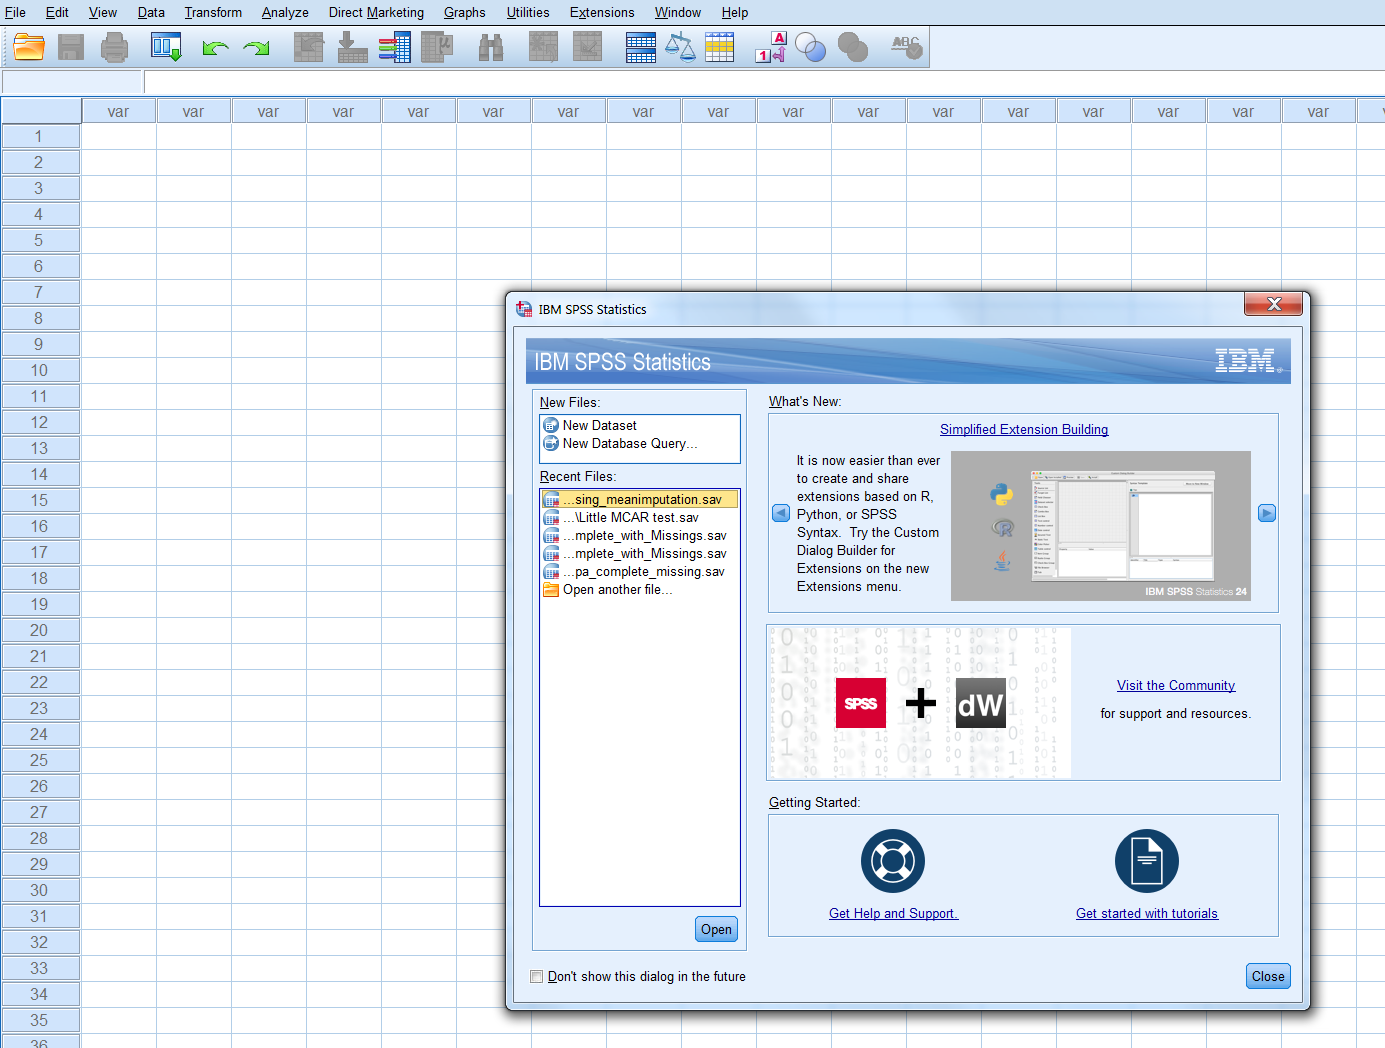
\includegraphics[width=0.9\linewidth]{images/fig1.1} 

}

\caption{First window after you have started SPSS}\label{fig:fig1}
\end{figure}

When you click on Close on the right side below, the window will close
and you will see an empty Data View window. Now you are in the SPSS Data
Editor window. This window is always open when you start SPSS. The name
``SPSS Data Editor'' is also visible at the top of the screen and is
called ``IBM SPSS Statistics Data Editor'' (Figure \ref{fig:fig2}).

\begin{figure}

{\centering 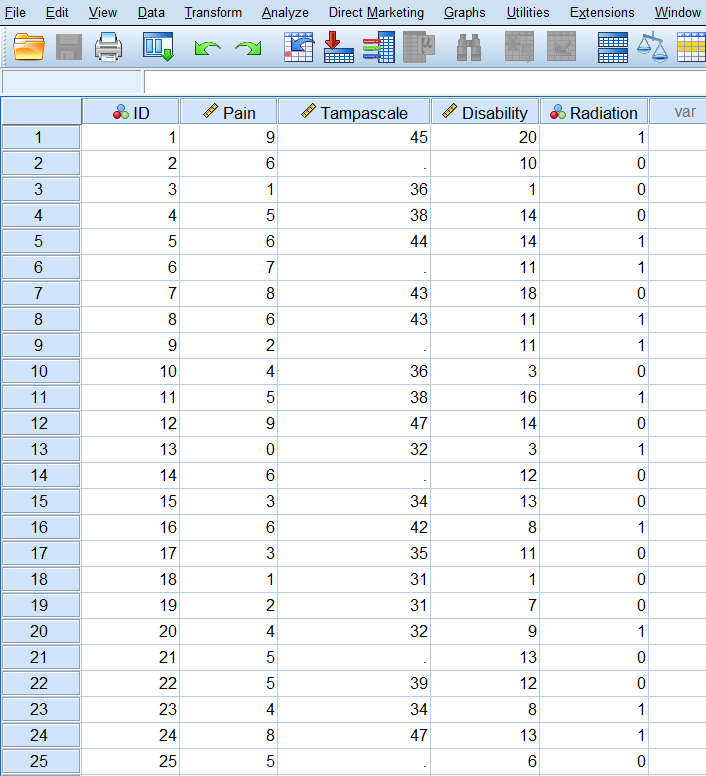
\includegraphics[width=0.9\linewidth]{images/fig1.2} 

}

\caption{Data View window in SPSS}\label{fig:fig2}
\end{figure}

In the SPSS Data Editor, you have the possibility to go to the Data View
and Variable View windows. In the Data View window, you can enter data
yourself or read in data by using the options in the file menu. In
Figure 1.2 you see an example of a dataset in the Data View window. Each
row in the Data View window represents a case and in the columns you
will find the variable names. In the Data View window, you can do all
kind of data manipulations by using the different menu's above in the
window. From here you can click on the tab Variable View, in the lower
left corner of the window. Than the Variable view window will appear
(Figure \ref{fig:fig3}).

\begin{figure}

{\centering 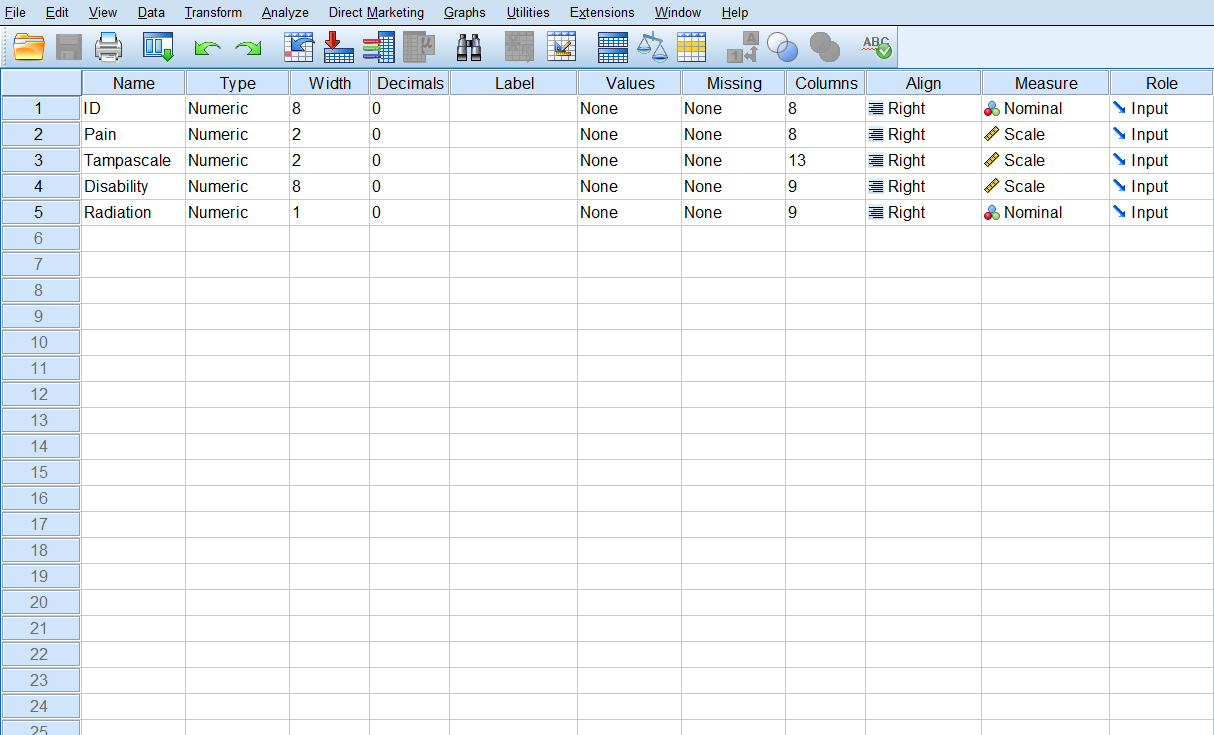
\includegraphics[width=0.9\linewidth]{images/fig1.3} 

}

\caption{Variable View window in SPSS}\label{fig:fig3}
\end{figure}

In the Variable View window, you can add new variables, by entering the
name in the name column. Further, you can change the columns by using
the following options: Type: Here you can change the type of variables
in your dataset. Mostly you work with numeric variables, i.e.~a variable
whose values are numbers. Other possibilities are Date variables which
is a numeric variable whose values are displayed in one of several
calendar-date or clock-time formats or String variables, a character
(text) variable that can contain any characters up to the defined
length. String values are not numeric and therefore are not used in
calculations. Width: By default SPSS defines a numeric variable with 8
digits for each new variable.

Decimals: the number of decimal places displayed.

Label: The variable name.

Values: To assign numbers to the categories of a variable. To define
Variable values do the following: 1. Click the button in the Values cell
for the variable that you want to define. 2. For each value, enter the
value and a label. 3. Click Add to enter the value label. 4. Click OK.

Missing: Here you can define specified data values as user-missing. You
can enter up to three discrete (individual) missing values, a range of
missing values, or a range plus one discrete value.

Columns: To change the number of characters displayed in the Data View
window.

Align: Here you can specify the alignment of your data.

Measure: Here you can specify the level of each variable, scale
(continuous), ordinal or nominal.

Role: Here you can define the role of the variable during your analysis.
Examples are, Input for independent variable, Target for dependent or
outcome variable, Both, independent and dependent variable. There are
more possibilities, but most of the times you use the default Input
setting.

\section{Analyzing data in SPSS}\label{analyzing-data-in-spss}

All statistical procedures in SPSS can be found under the Analyze button
(Figure \ref{fig:fig4}). Here you also will find the option ``Multiple
Imputation'' which plays an important role in this manual. We will use
this menu later on in Chapter 4.

\begin{figure}

{\centering 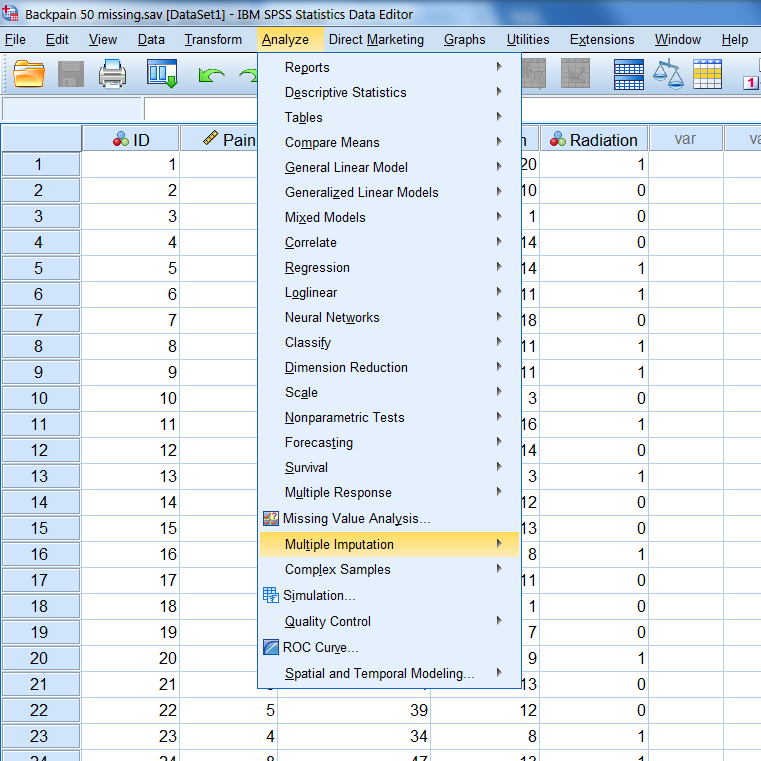
\includegraphics[width=0.9\linewidth]{images/fig1.4} 

}

\caption{Statistical procedures that can be found under the Analyze menu in SPSS}\label{fig:fig4}
\end{figure}

\section{Data Transformations in
SPSS}\label{data-transformations-in-spss}

Two other interesting buttons are Data and Transform. The Data menu
allows you to make changes to the data editor. Here you can add new
variables or cases. You can also use the Split File option, to get
analyses results separately for categories of a variable. The Transform
menu allows you to manipulate your variables by for example
dichotomizing a numeric variable.

\section{The Output window in SPSS}\label{the-output-window-in-spss}

If you have run your analyses in SPSS, an SPSS Output (or viewer) Window
will pop-up. The main body of the Output Window consists of two panes
(left and right panes). In the left pane you will find an outline of the
output. In the right pane you will find the actual output of your
statistical procedure (Figure \ref{fig:fig5}).

\begin{figure}

{\centering 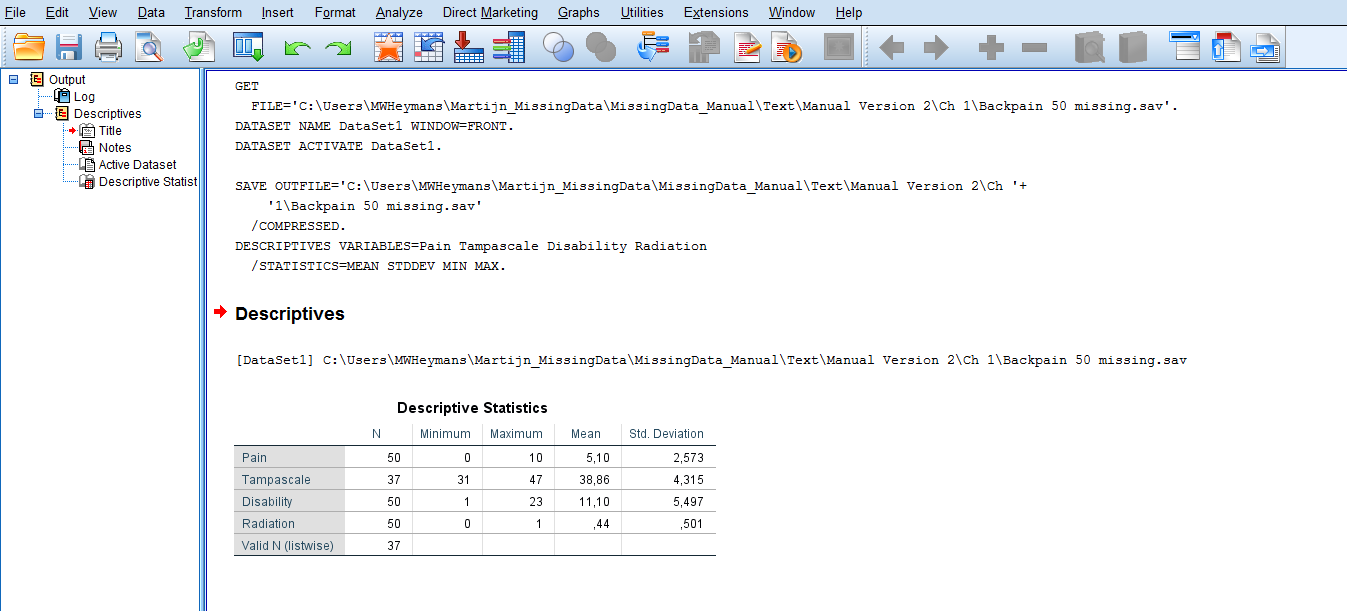
\includegraphics[width=0.9\linewidth]{images/fig1.5} 

}

\caption{Part of the Output or Viewer window in SPSS after making use of Descriptive Statistics under the Analyze menu}\label{fig:fig5}
\end{figure}

\section{The Syntax Editor in SPSS}\label{the-syntax-editor-in-spss}

In the syntax editor of SPSS, you use the SPSS syntax programming
language. You can run all SPSS procedures by typing in commands in this
syntax editor window, instead of using the graphical user interface,
i.e.~by using your mouse and clicking on the menu´s. You can get access
to the syntax window in two ways. The first is just by opening a new
syntax file by navigating to File -\textgreater{} New -\textgreater{}
Syntax. This will open a new syntax window (Figure \ref{fig:fig6}).

\begin{figure}

{\centering 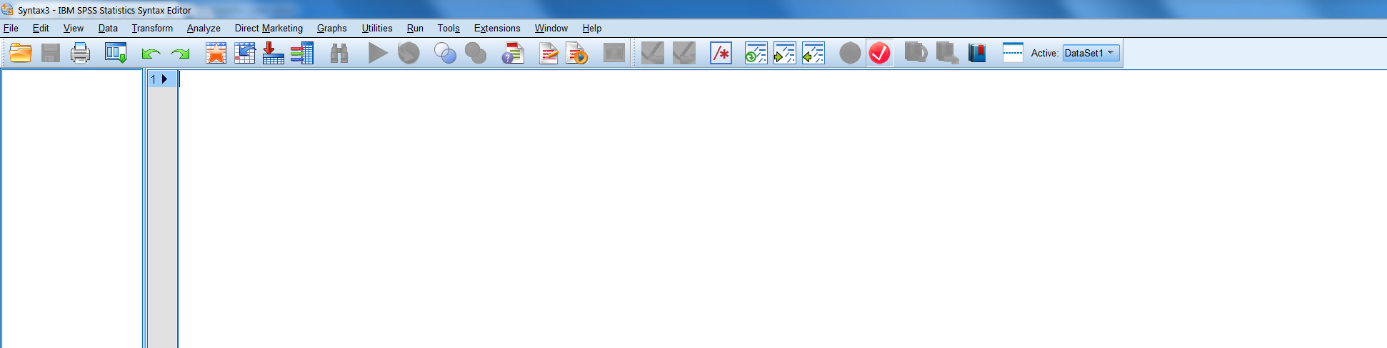
\includegraphics[width=0.9\linewidth]{images/fig1.6} 

}

\caption{Screenshot of new syntax file}\label{fig:fig6}
\end{figure}

Now you can start writing your syntax directly in this window. You can
also generate syntax by accessing statistical procedures through the
dropdown menus and clicking the Paste button instead of clicking the OK
button after you have specified the options. When you have clicked the
Paste button, a new Syntax Editor window will pop up or the new syntax
will automatically be added to the open Syntax Editor window. This is a
very useful way to keep track of the analysis that you have performed.
An example can be found in Figure \ref{fig:fig7}, where the syntax is
shown for the Descriptive Statistics procedure of Figure \ref{fig:fig5}.

\begin{figure}

{\centering 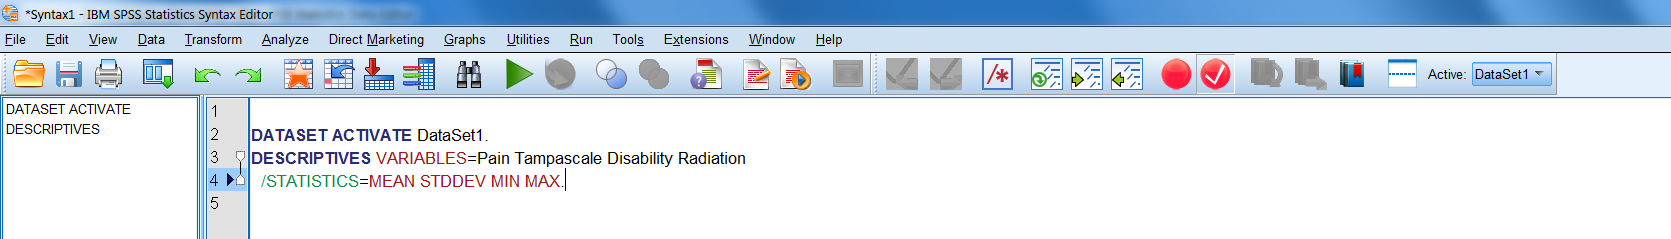
\includegraphics[width=0.9\linewidth]{images/fig1.7} 

}

\caption{Screenshot of Syntax editor of SPSS including the Syntax code for descriptive statisitcs}\label{fig:fig7}
\end{figure}

By using the SPSS Syntax it is possible for users to perform the same
analyses over and over again or to adapt the analysis via the syntax
code for complex calculations in the data. In this manual we will not
use SPSS syntax code to access statistical procedures, however we
recommend to use the SPSS syntax to keep track of the analysis that you
have performed. SPSS is most frequently used via the graphical user
interface, and we will use that method also in this manual.

\section{Reading and saving data in
SPSS}\label{reading-and-saving-data-in-spss}

Reading in data in SPSS is very easy; via the menu File choose for File
-\textgreater{} Open -\textgreater{} Data. All kind of file types can be
selected. Of course the SPSS .sav files, but also .por, .xlsx, .cvs,
SAS, Stata, etc. (Figure 1.8). After you have selected a specific file
type you may have to go through several steps before you see the data in
the Data View window. These steps are not necessary for SPSS files, they
open directly in the data editor.

\begin{figure}

{\centering 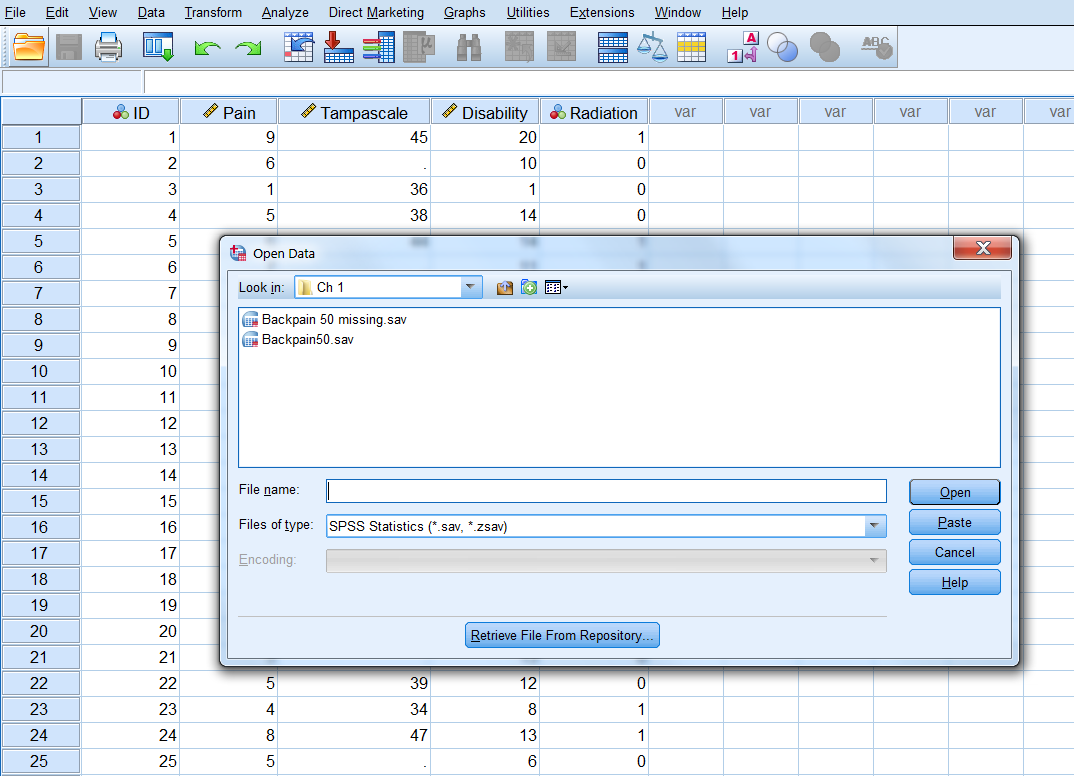
\includegraphics[width=0.9\linewidth]{images/fig1.8} 

}

\caption{Window to read in different file types in SPSS}\label{fig:fig8}
\end{figure}

Saving files in SPSS is possible via the Save Data As option under the
menu File. You can choose the same kind of file types (Figure
\ref{fig:fig9}).

\begin{figure}

{\centering 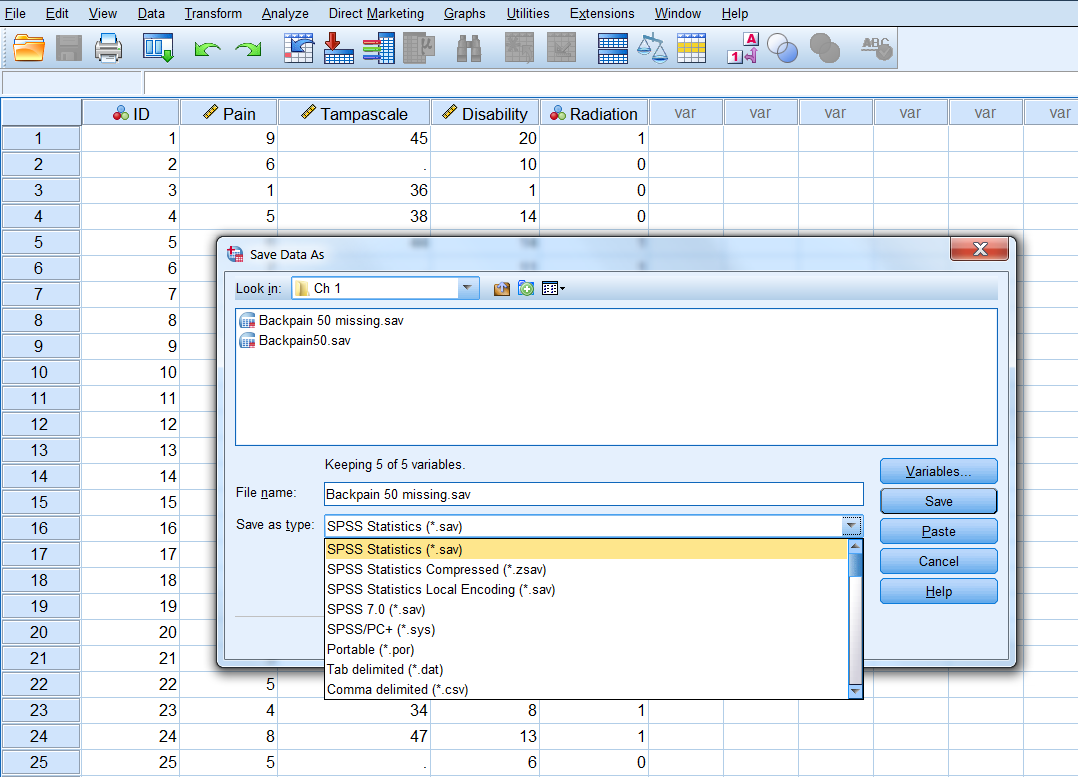
\includegraphics[width=0.9\linewidth]{images/fig1.9} 

}

\caption{Option Save Data As under the menu File}\label{fig:fig9}
\end{figure}

\section{R and RStudio}\label{r-and-rstudio}

RStudio is an integrated environment to work with the software program
R. Consequently, to work with RStudio, R has to be installed. RStudio
uses the R language and is also freely available. In this manual we will
only show some possibilities and options in RStudio that are needed to
run the R code and the programs that are discussed in this manual. For
more information about RStudio and its possibilities visit the RStudio
website at www.rstudio.com. When you open RStudio the following screen
will appear.

\begin{figure}

{\centering 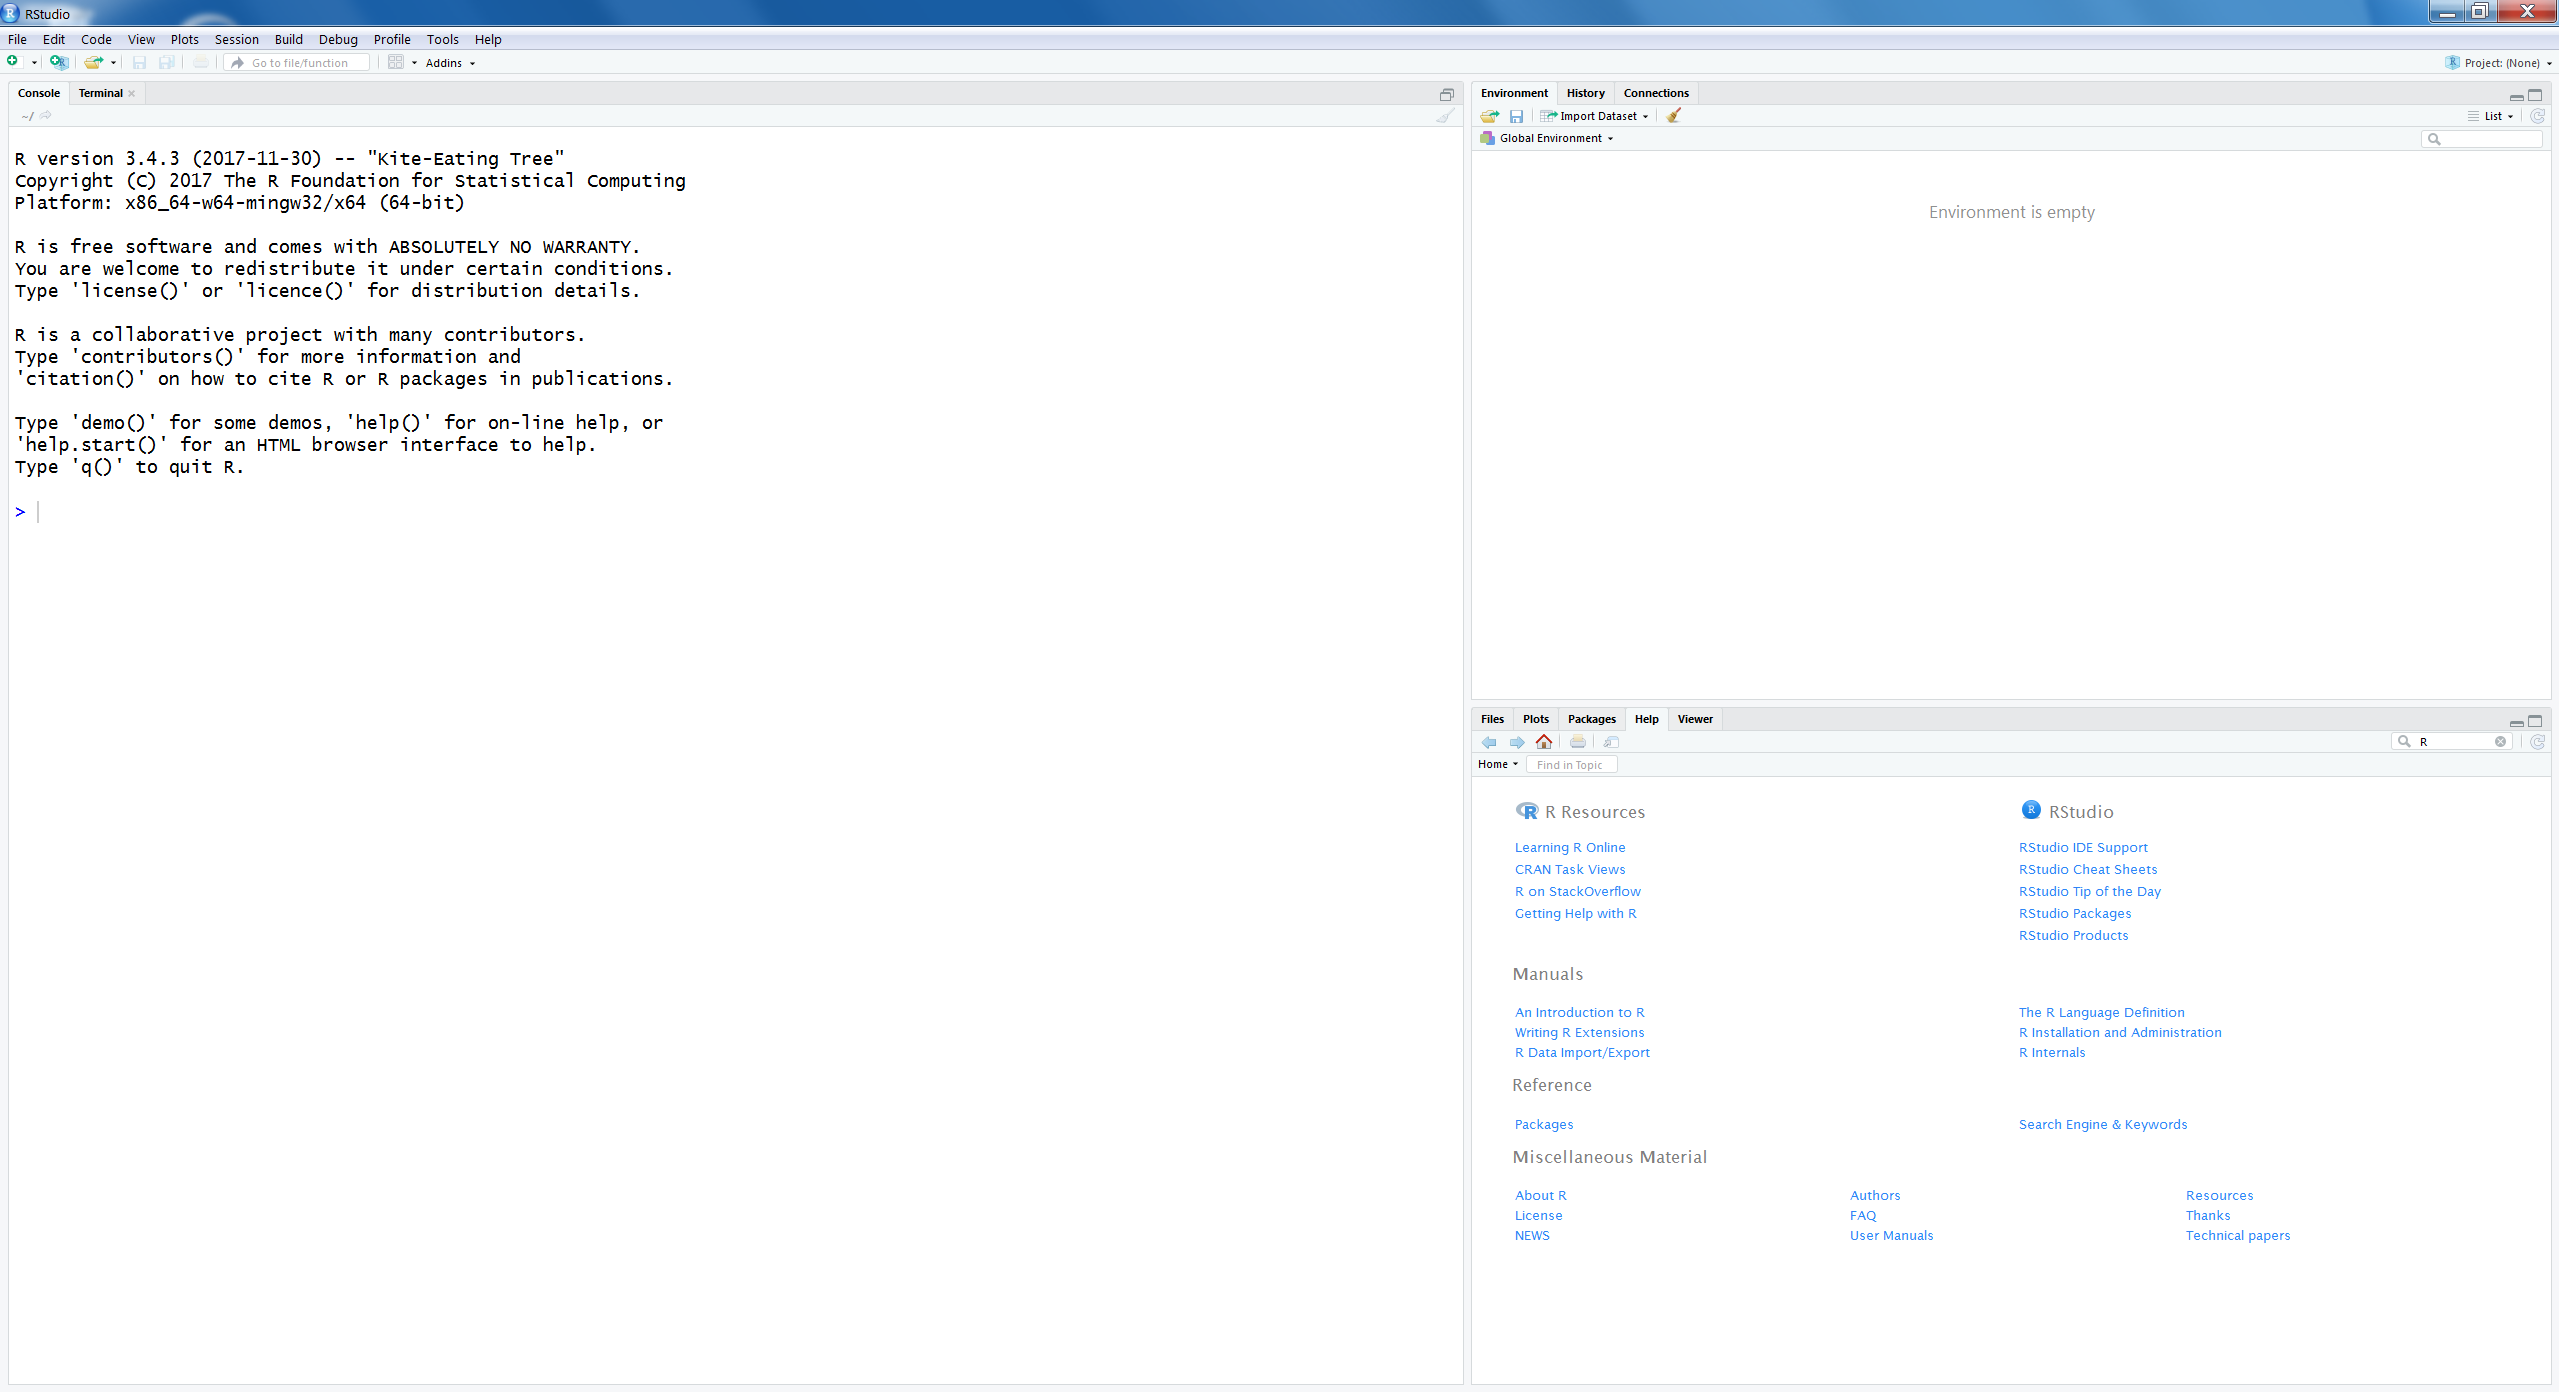
\includegraphics[width=0.9\linewidth]{images/fig1.10} 

}

\caption{First screen that appears after you have started RStudio}\label{fig:fig10}
\end{figure}

There are three windows opened:

\begin{enumerate}
\def\labelenumi{\arabic{enumi}.}
\tightlist
\item
  On the left is the Console window
\end{enumerate}

This is the main window to run R code (see below for more information
about the Console window).

\begin{enumerate}
\def\labelenumi{\arabic{enumi}.}
\setcounter{enumi}{1}
\tightlist
\item
  Right above is the window where you can choose between the Environment
  and History tabs (e.g.~history tracks the code you typed in the
  Console window).
\item
  At the right site below is the window where you can choose between
  Files, Plots, Packages, Help and Viewer tabs.
\end{enumerate}

When you enter code in the Console window you will directly receive a
result. For example, you can type the following code and the result will
appear directly in the Console window.

\textbf{R code 1.1}

\begin{Shaded}
\begin{Highlighting}[]
\DecValTok{3} \OperatorTok{+}\StringTok{ }\DecValTok{3}
\end{Highlighting}
\end{Shaded}

\begin{verbatim}
## [1] 6
\end{verbatim}

\begin{figure}

{\centering 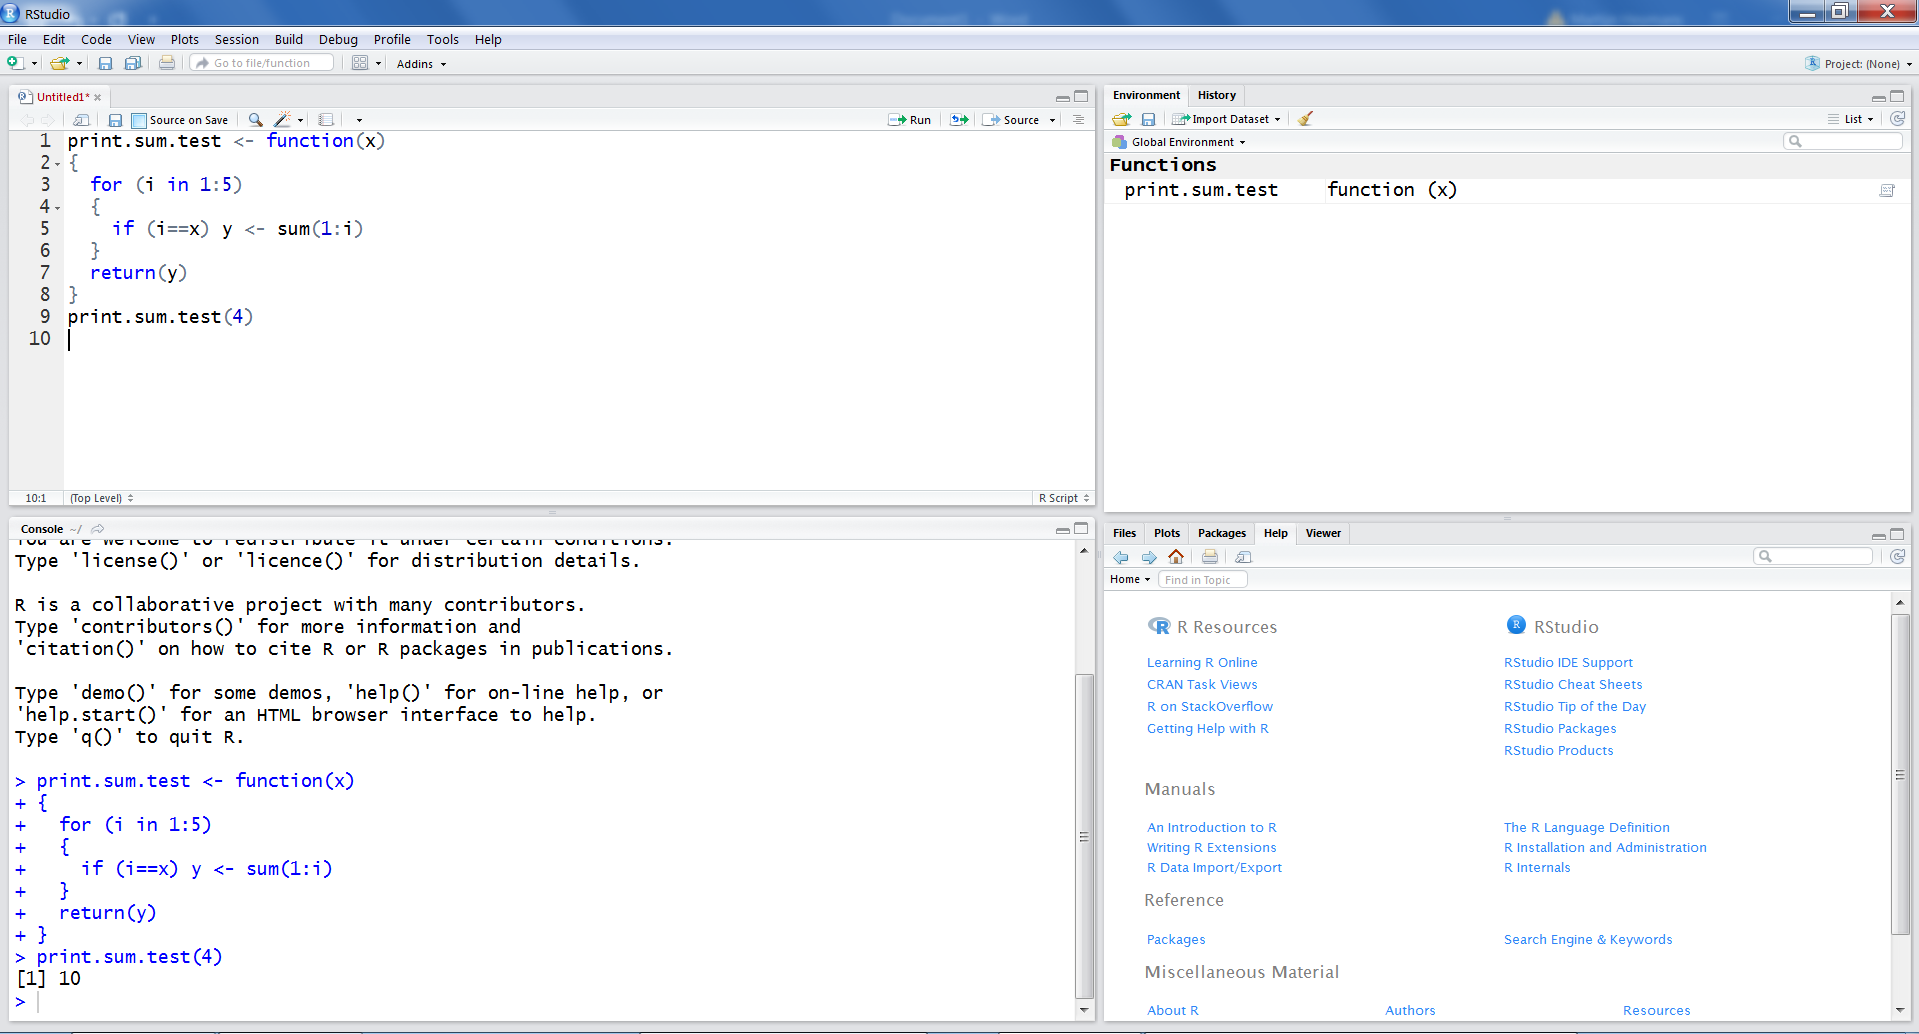
\includegraphics[width=0.9\linewidth]{images/fig1.11} 

}

\caption{Script file example in RStudio}\label{fig:fig11}
\end{figure}

\begin{figure}

{\centering 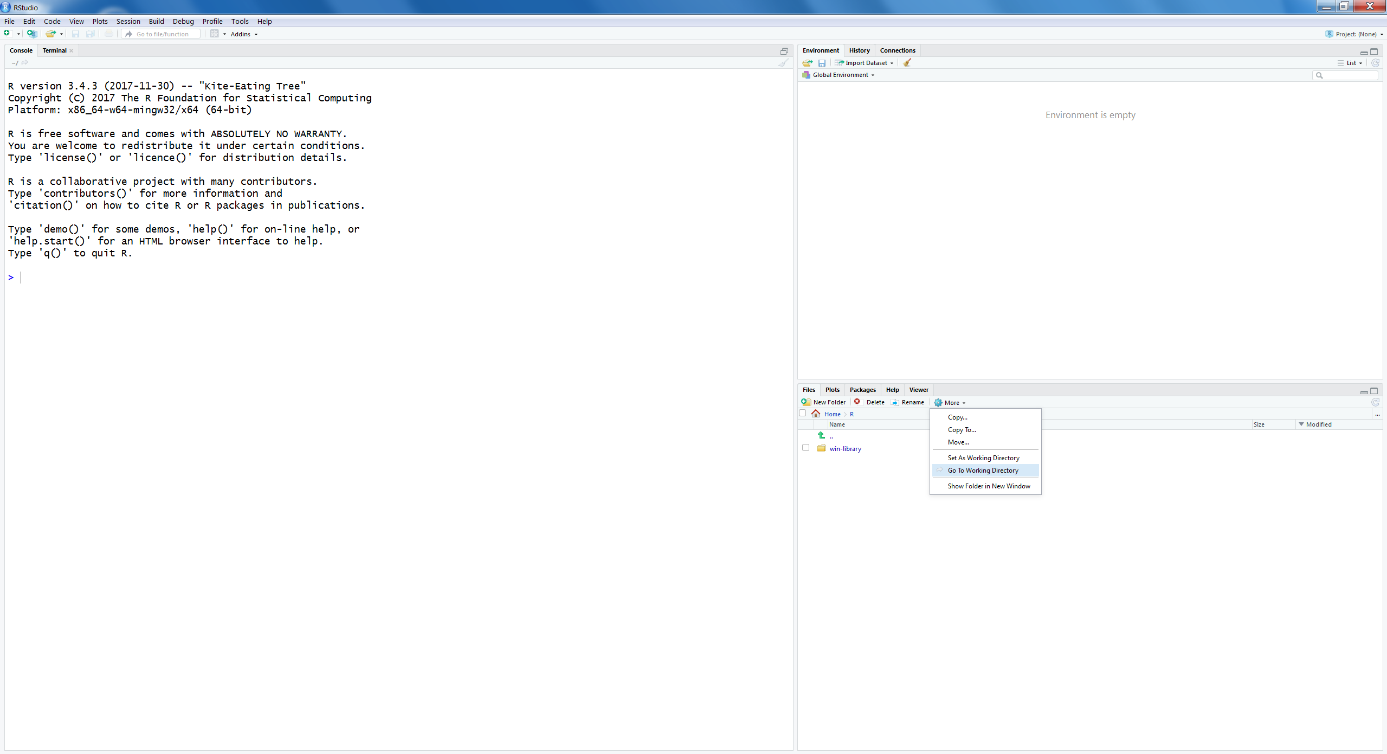
\includegraphics[width=0.9\linewidth]{images/fig1.12} 

}

\caption{Working directory selection in RStudio}\label{fig:fig12}
\end{figure}

\begin{figure}

{\centering 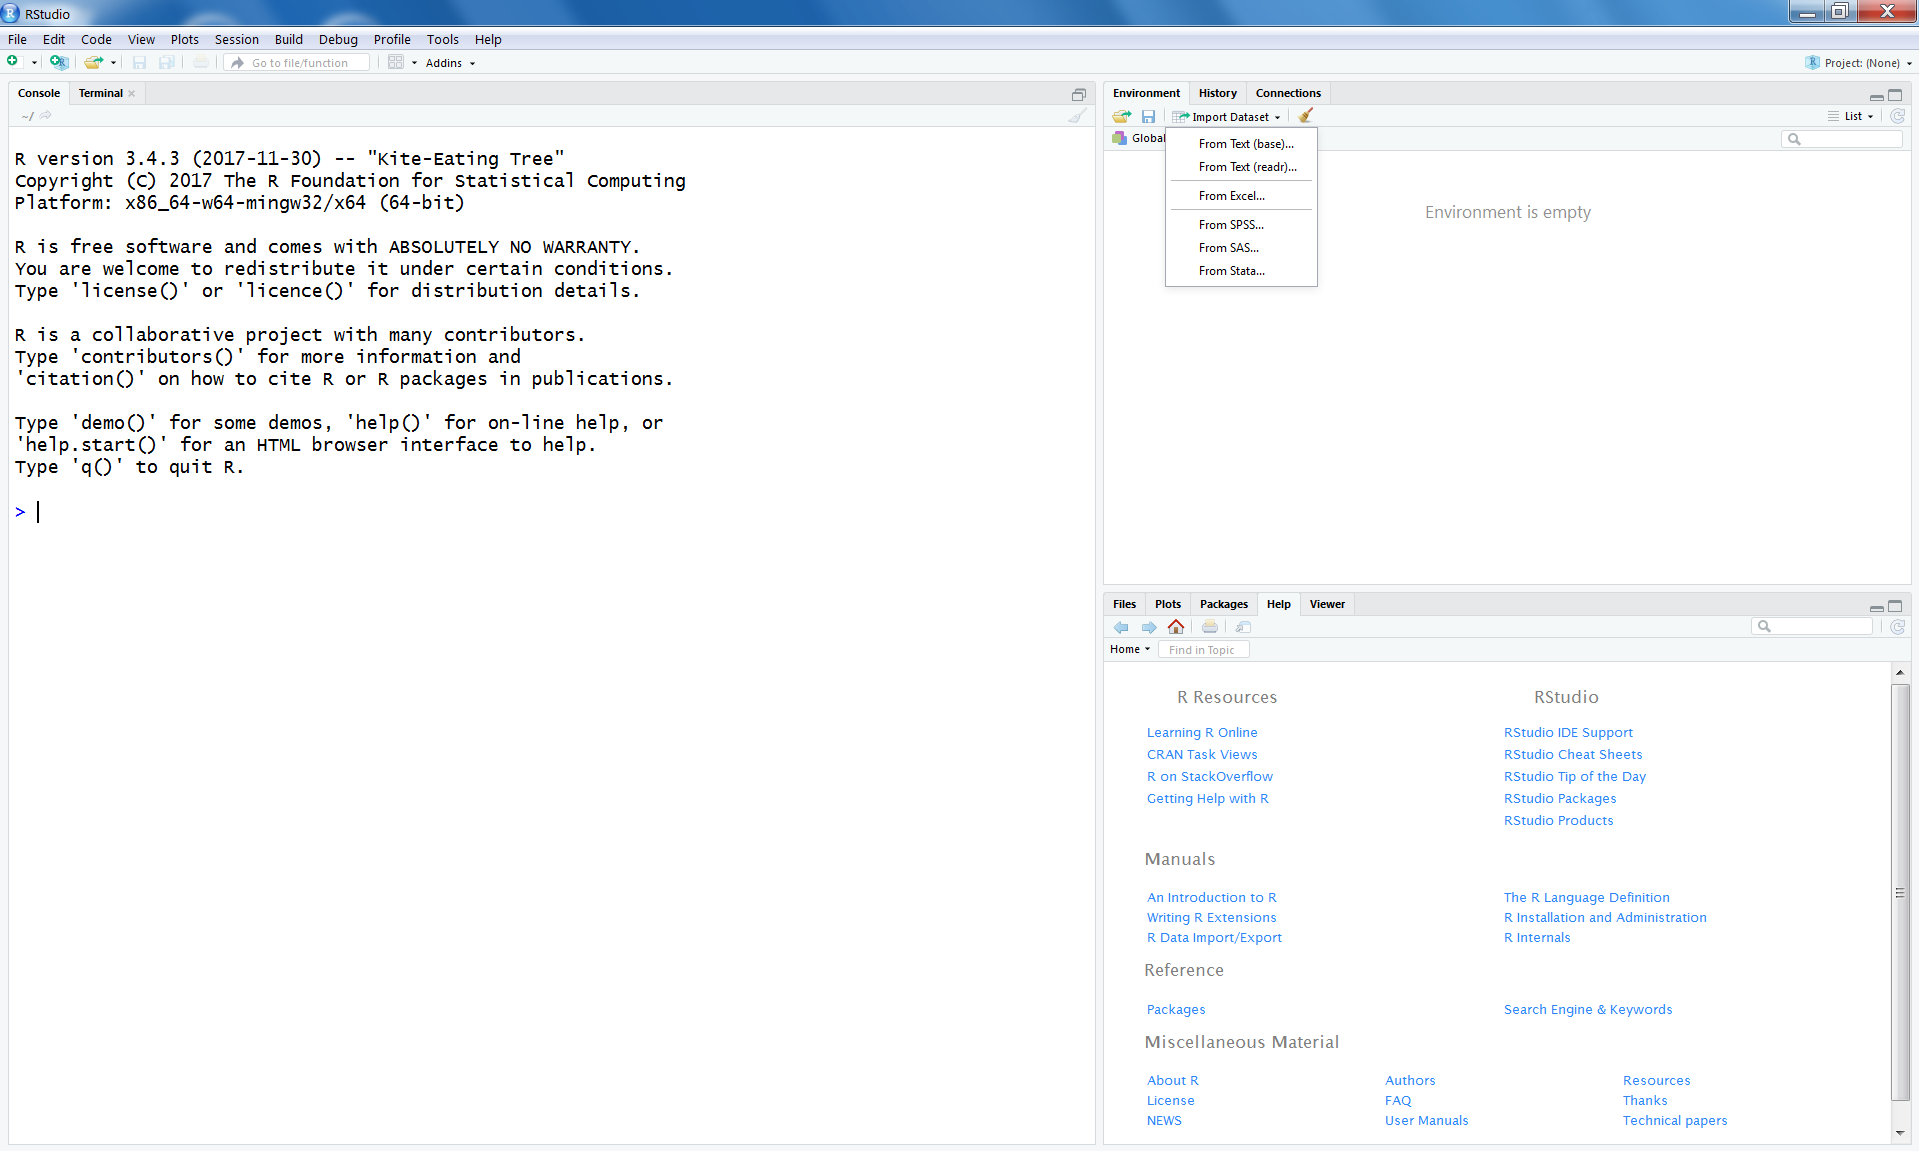
\includegraphics[width=0.9\linewidth]{images/fig1.13} 

}

\caption{Screen to import datasets in RStudio}\label{fig:fig13}
\end{figure}

\begin{figure}

{\centering 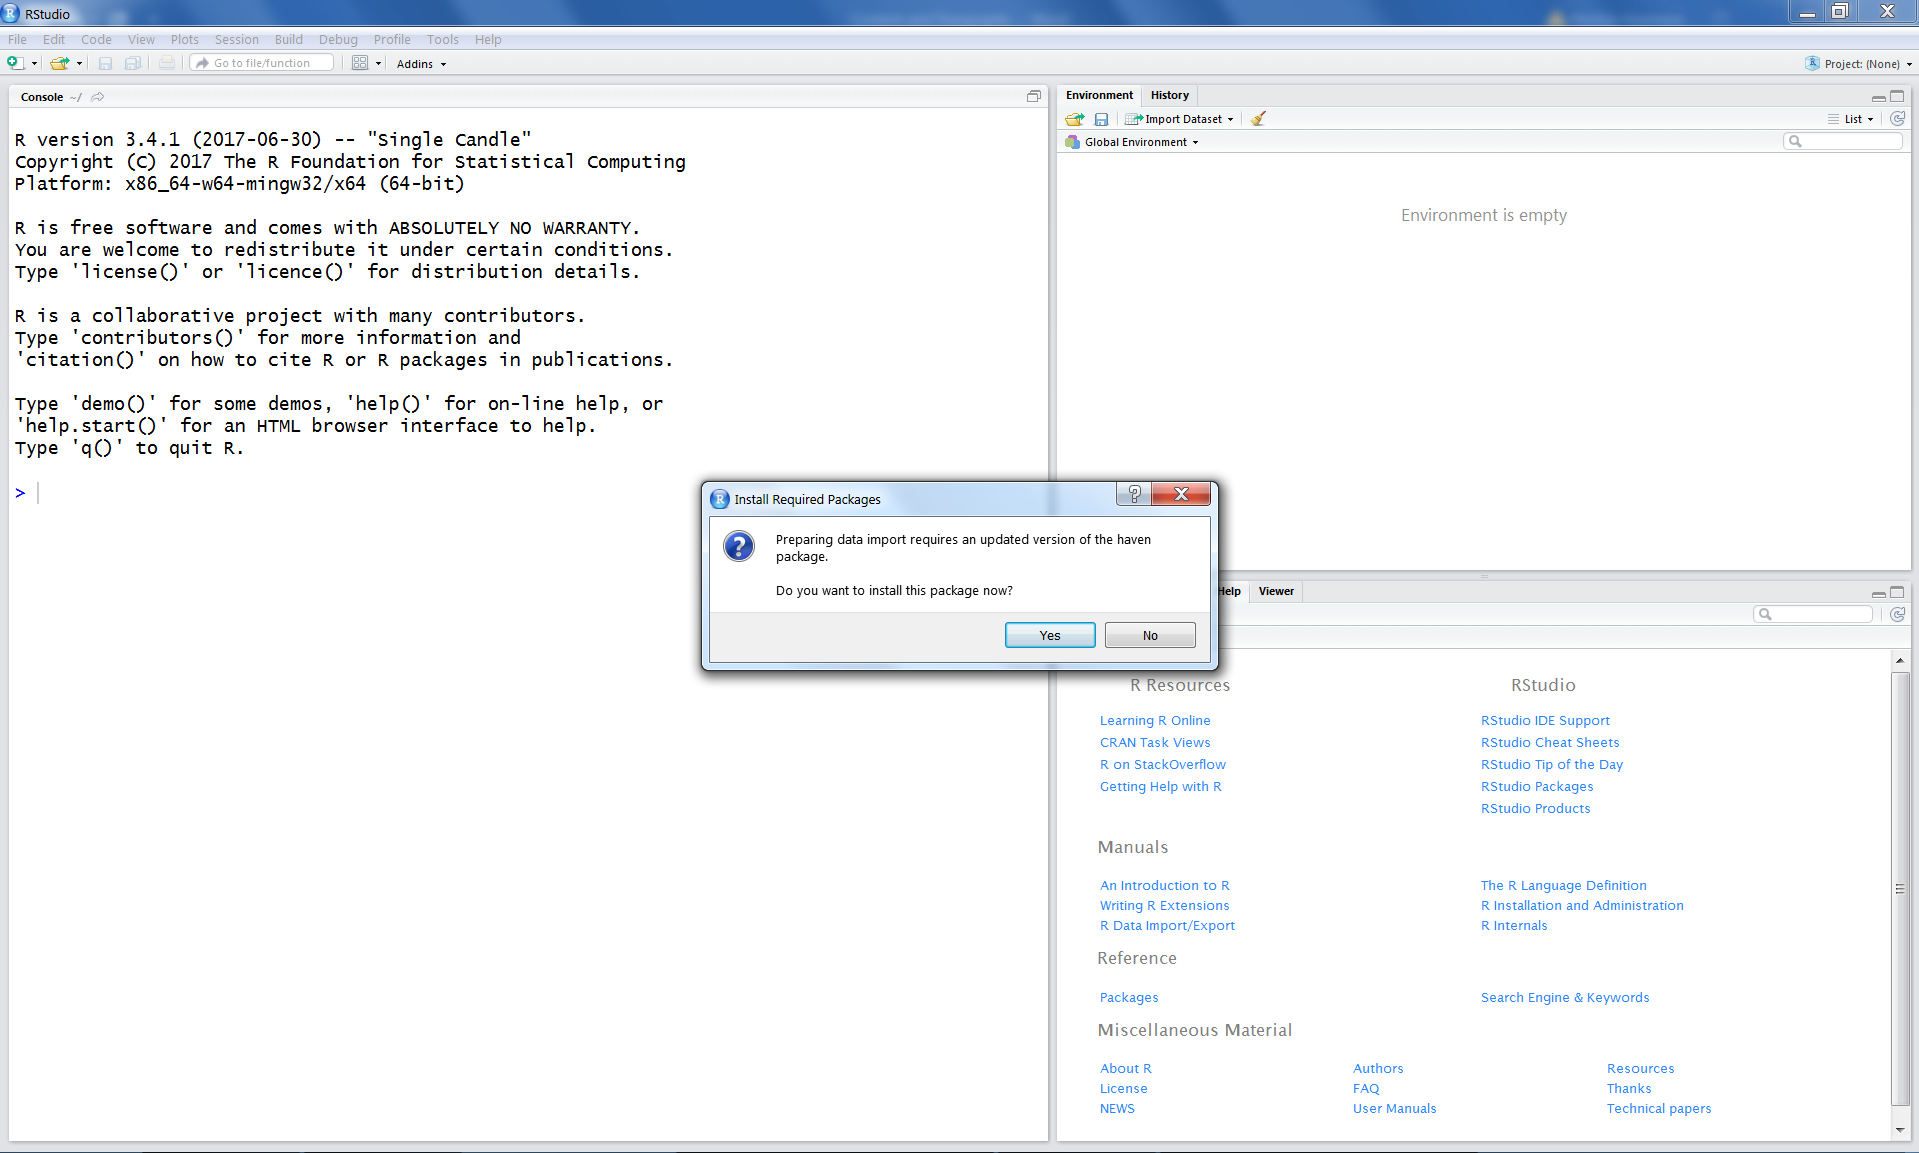
\includegraphics[width=0.9\linewidth]{images/fig1.14} 

}

\caption{Window to install the haven package}\label{fig:fig14}
\end{figure}

\begin{figure}

{\centering 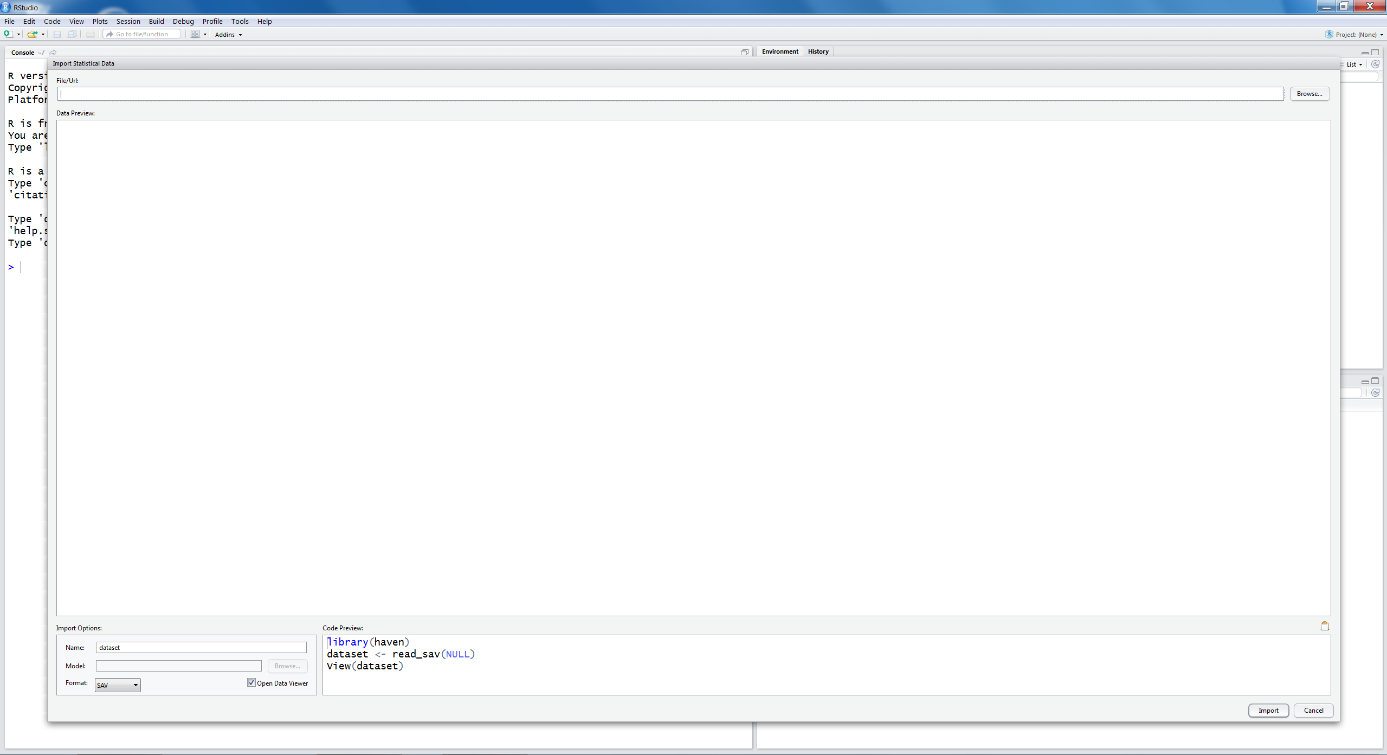
\includegraphics[width=0.9\linewidth]{images/fig1.15} 

}

\caption{The Import Statistical Data window in RStudio}\label{fig:fig15}
\end{figure}

\begin{figure}

{\centering 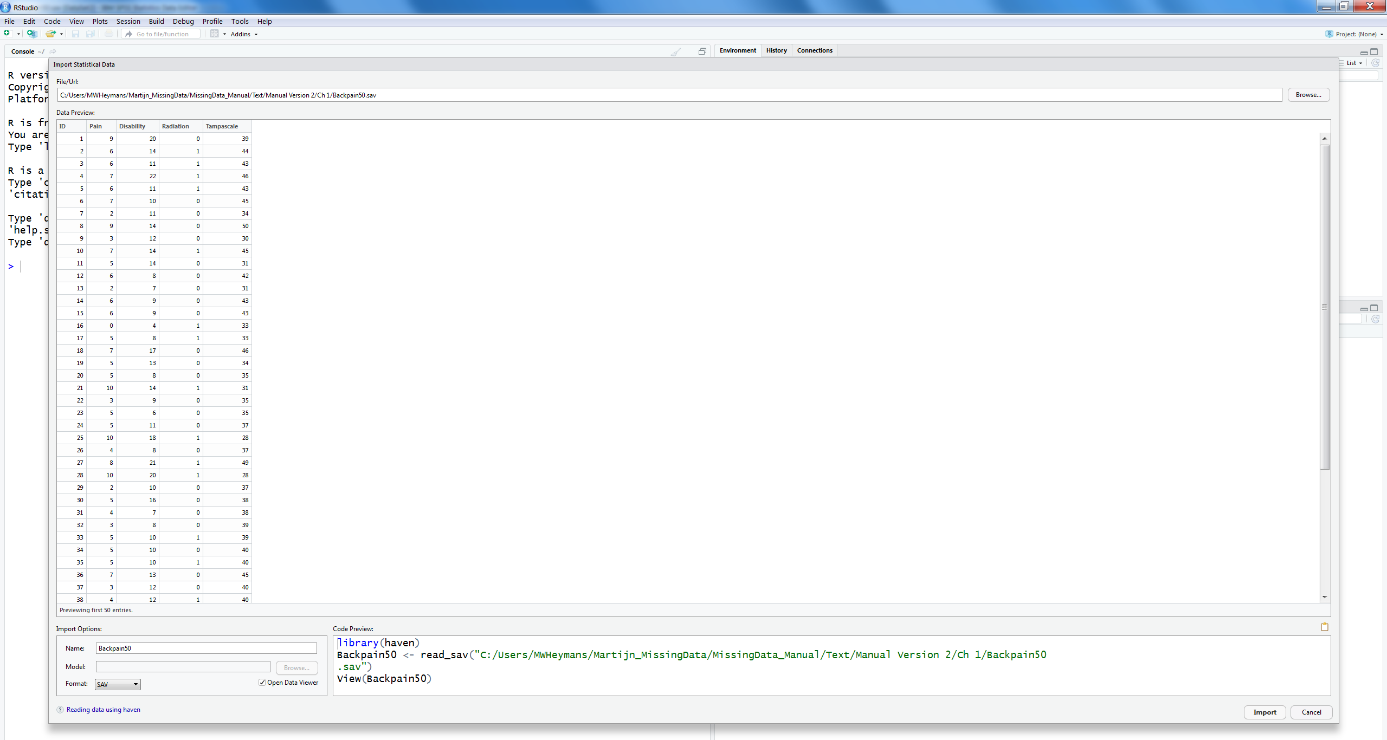
\includegraphics[width=0.9\linewidth]{images/fig1.16} 

}

\caption{A preview of the dataset in RStudio}\label{fig:fig16}
\end{figure}

\begin{figure}

{\centering 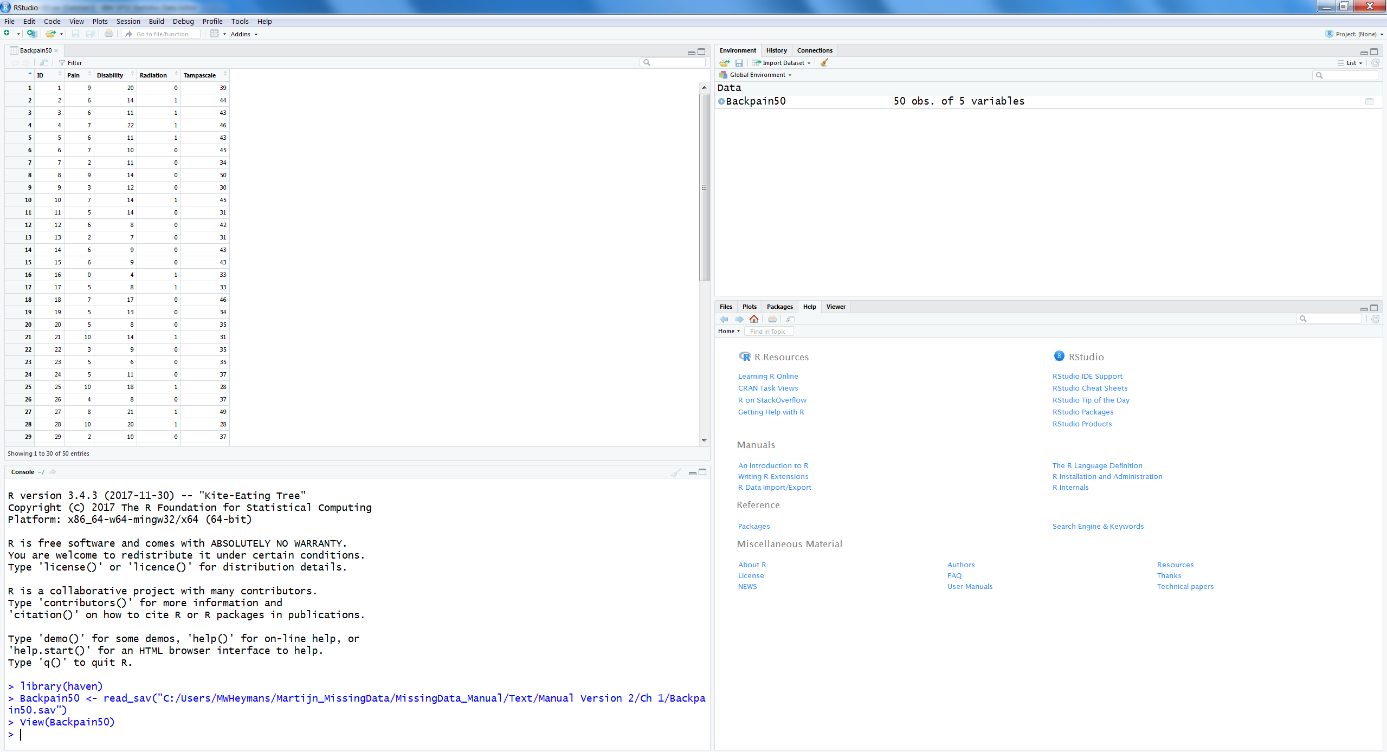
\includegraphics[width=0.9\linewidth]{images/fig1.17} 

}

\caption{Imported dataset in RStudio}\label{fig:fig17}
\end{figure}

\begin{figure}

{\centering 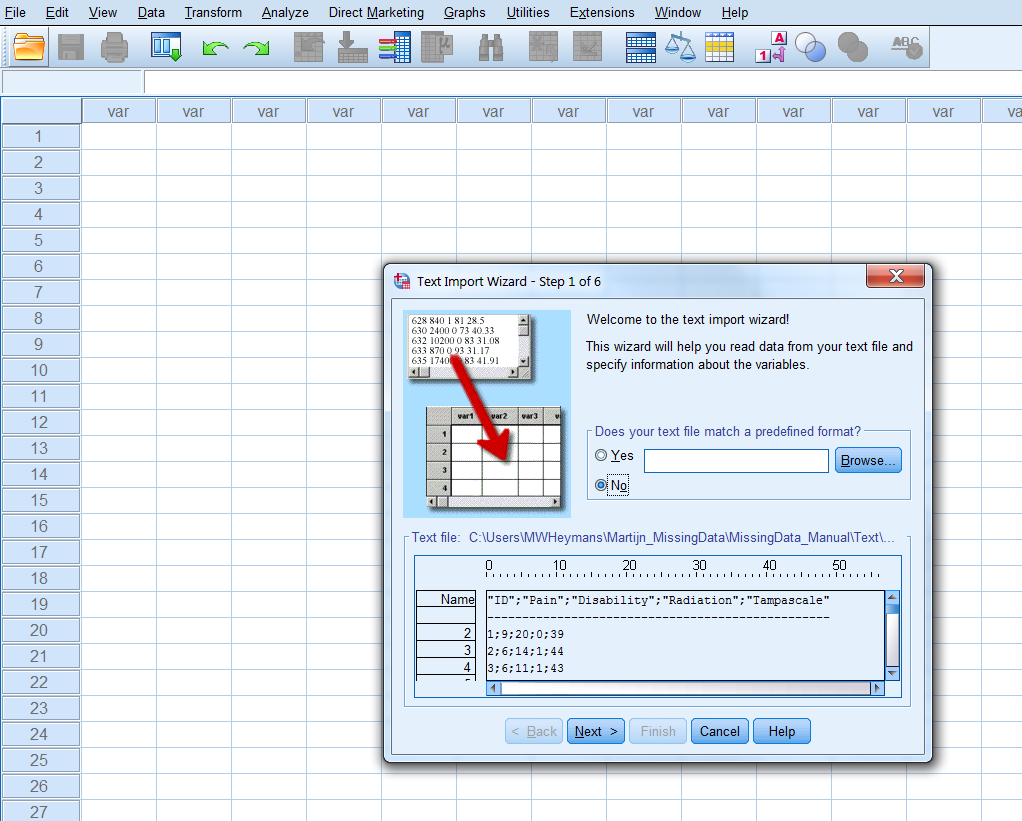
\includegraphics[width=0.9\linewidth]{images/fig1.19} 

}

\caption{Step 1 of the Text Import Wizard}\label{fig:fig19}
\end{figure}

\begin{figure}

{\centering 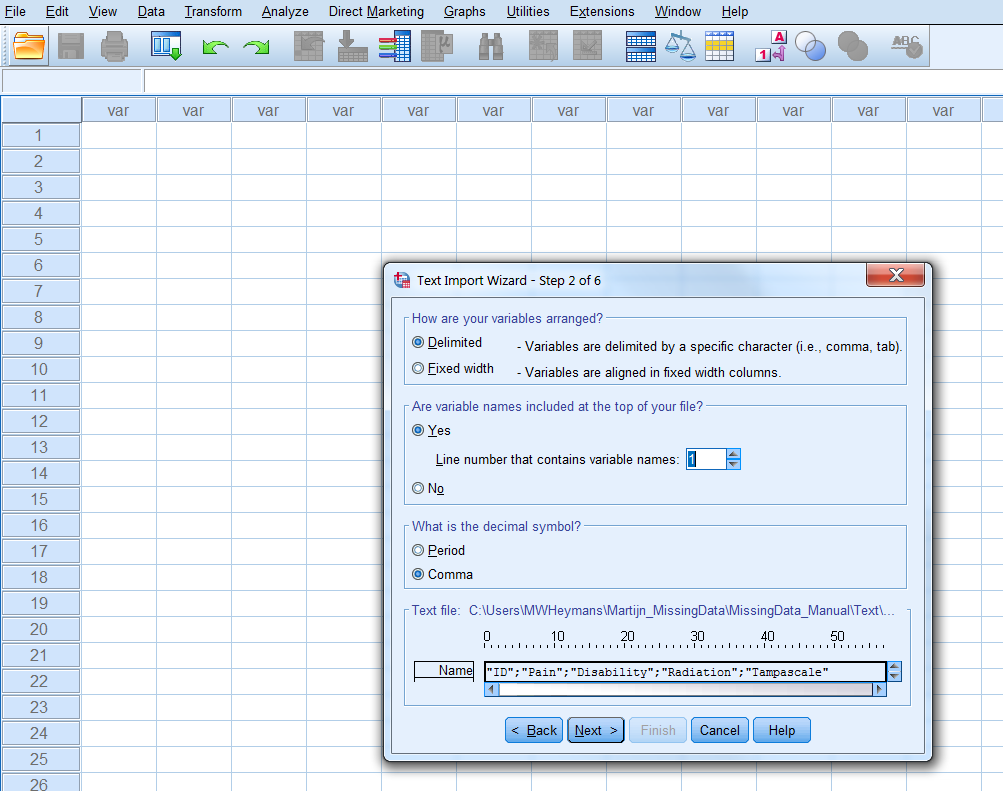
\includegraphics[width=0.9\linewidth]{images/fig1.20} 

}

\caption{Step 2 of the Text Import Wizard}\label{fig:fig20}
\end{figure}

\begin{figure}

{\centering 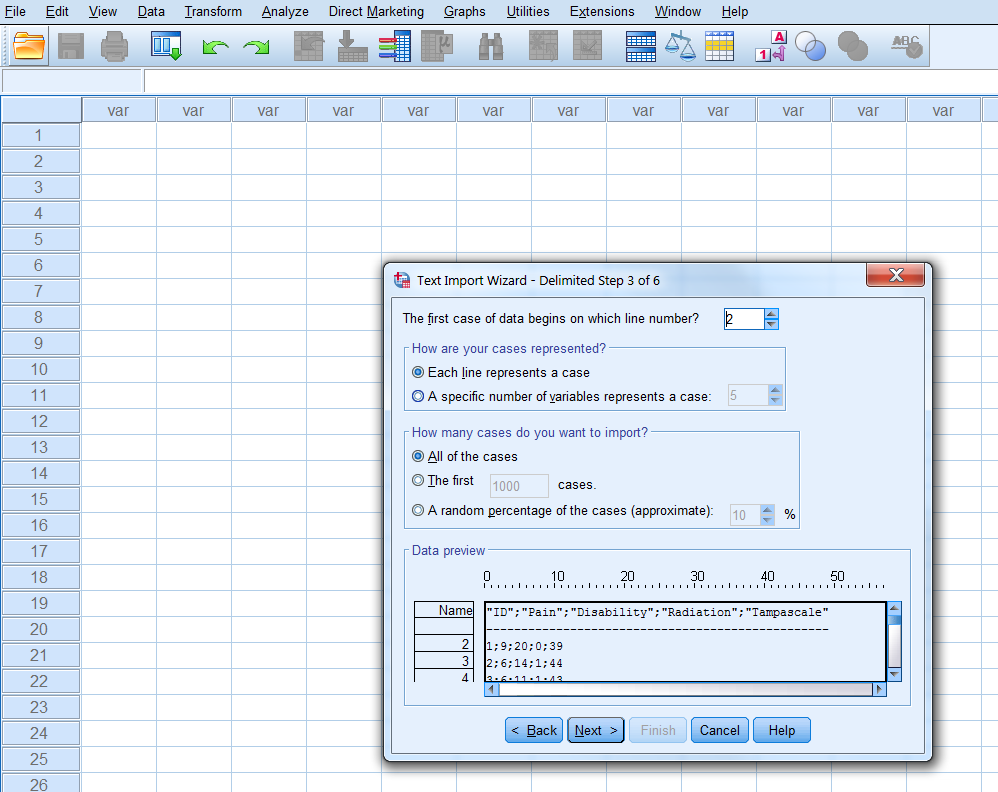
\includegraphics[width=0.9\linewidth]{images/fig1.21} 

}

\caption{Step 3 of the Text Import Wizard}\label{fig:fig21}
\end{figure}

\begin{figure}

{\centering 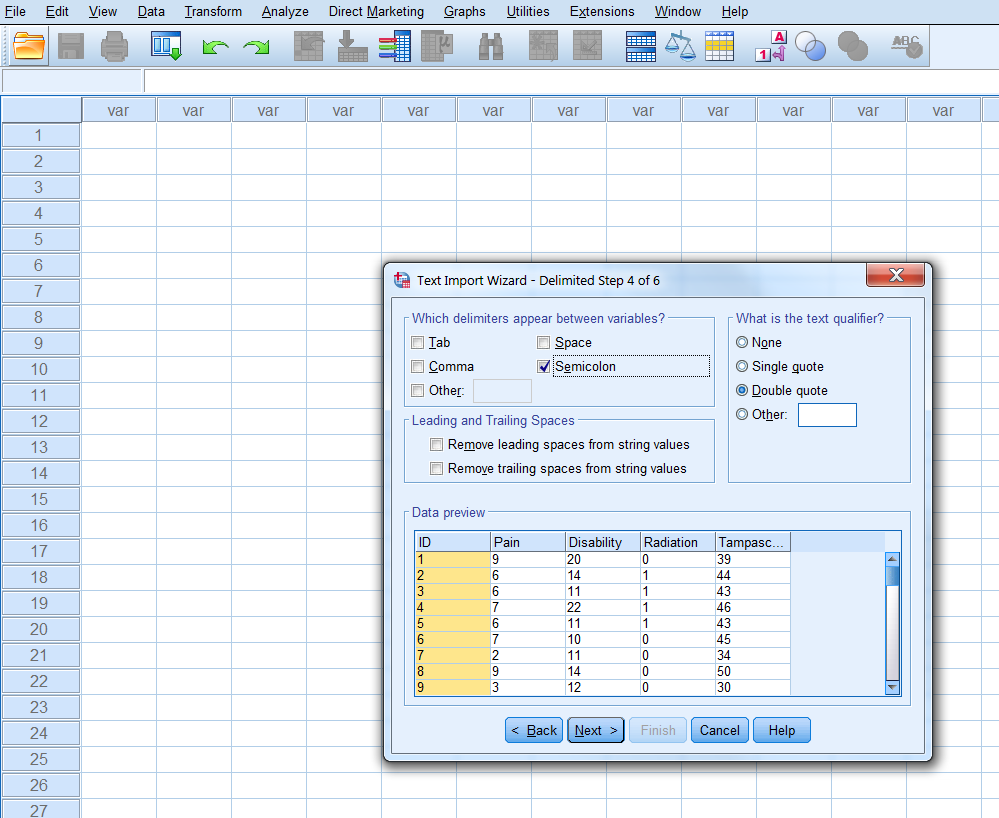
\includegraphics[width=0.9\linewidth]{images/fig1.22} 

}

\caption{Step 4 of the Text Import Wizard}\label{fig:fig22}
\end{figure}

\begin{figure}

{\centering 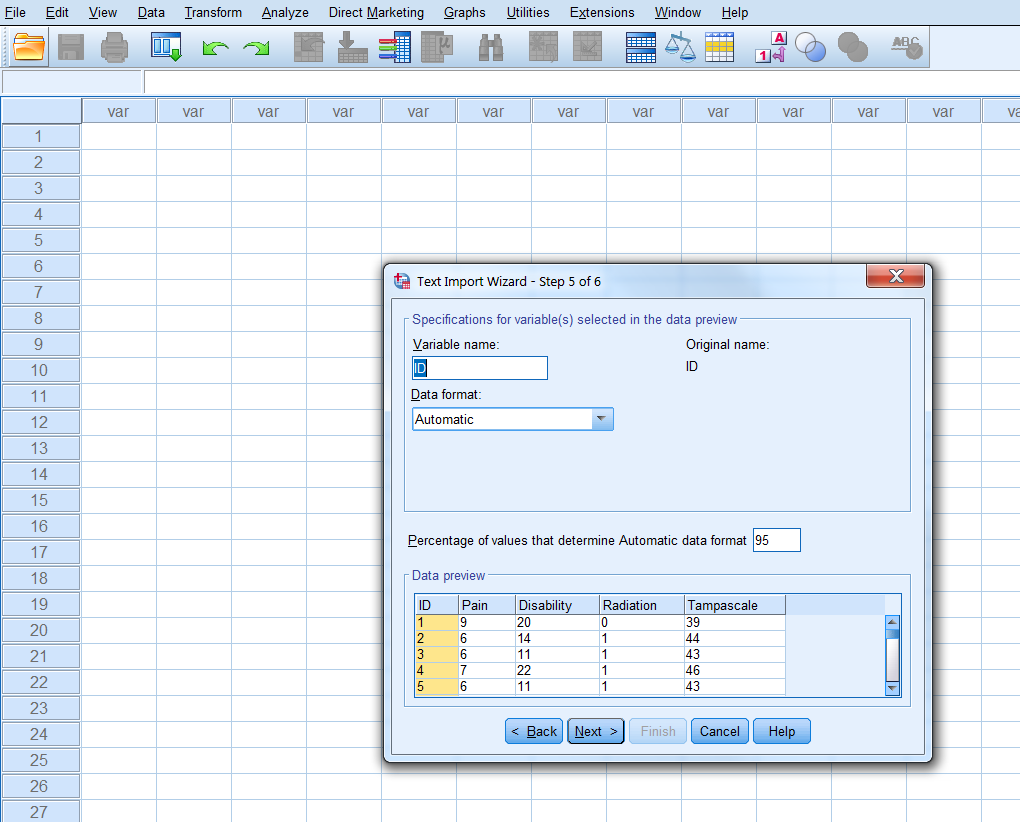
\includegraphics[width=0.9\linewidth]{images/fig1.23} 

}

\caption{Step 5 of the Text Import Wizard}\label{fig:fig23}
\end{figure}

\begin{figure}

{\centering 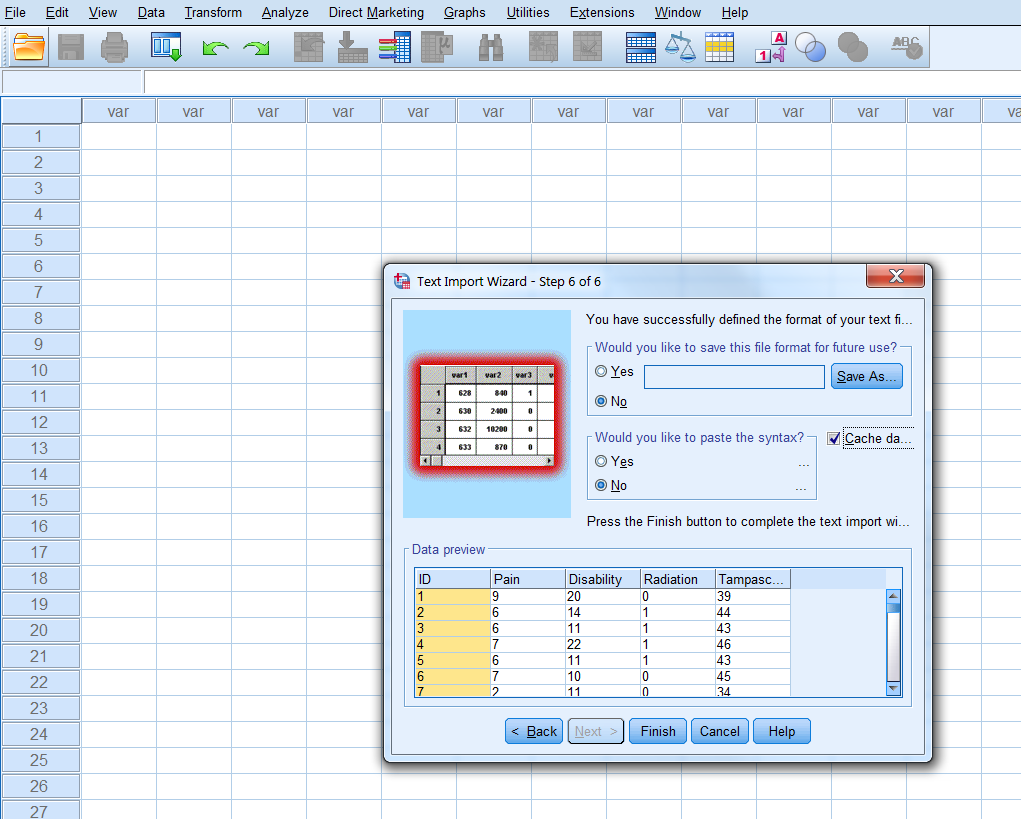
\includegraphics[width=0.9\linewidth]{images/fig1.24} 

}

\caption{Step 6 of the Text Import Wizard}\label{fig:fig24}
\end{figure}

\begin{figure}

{\centering 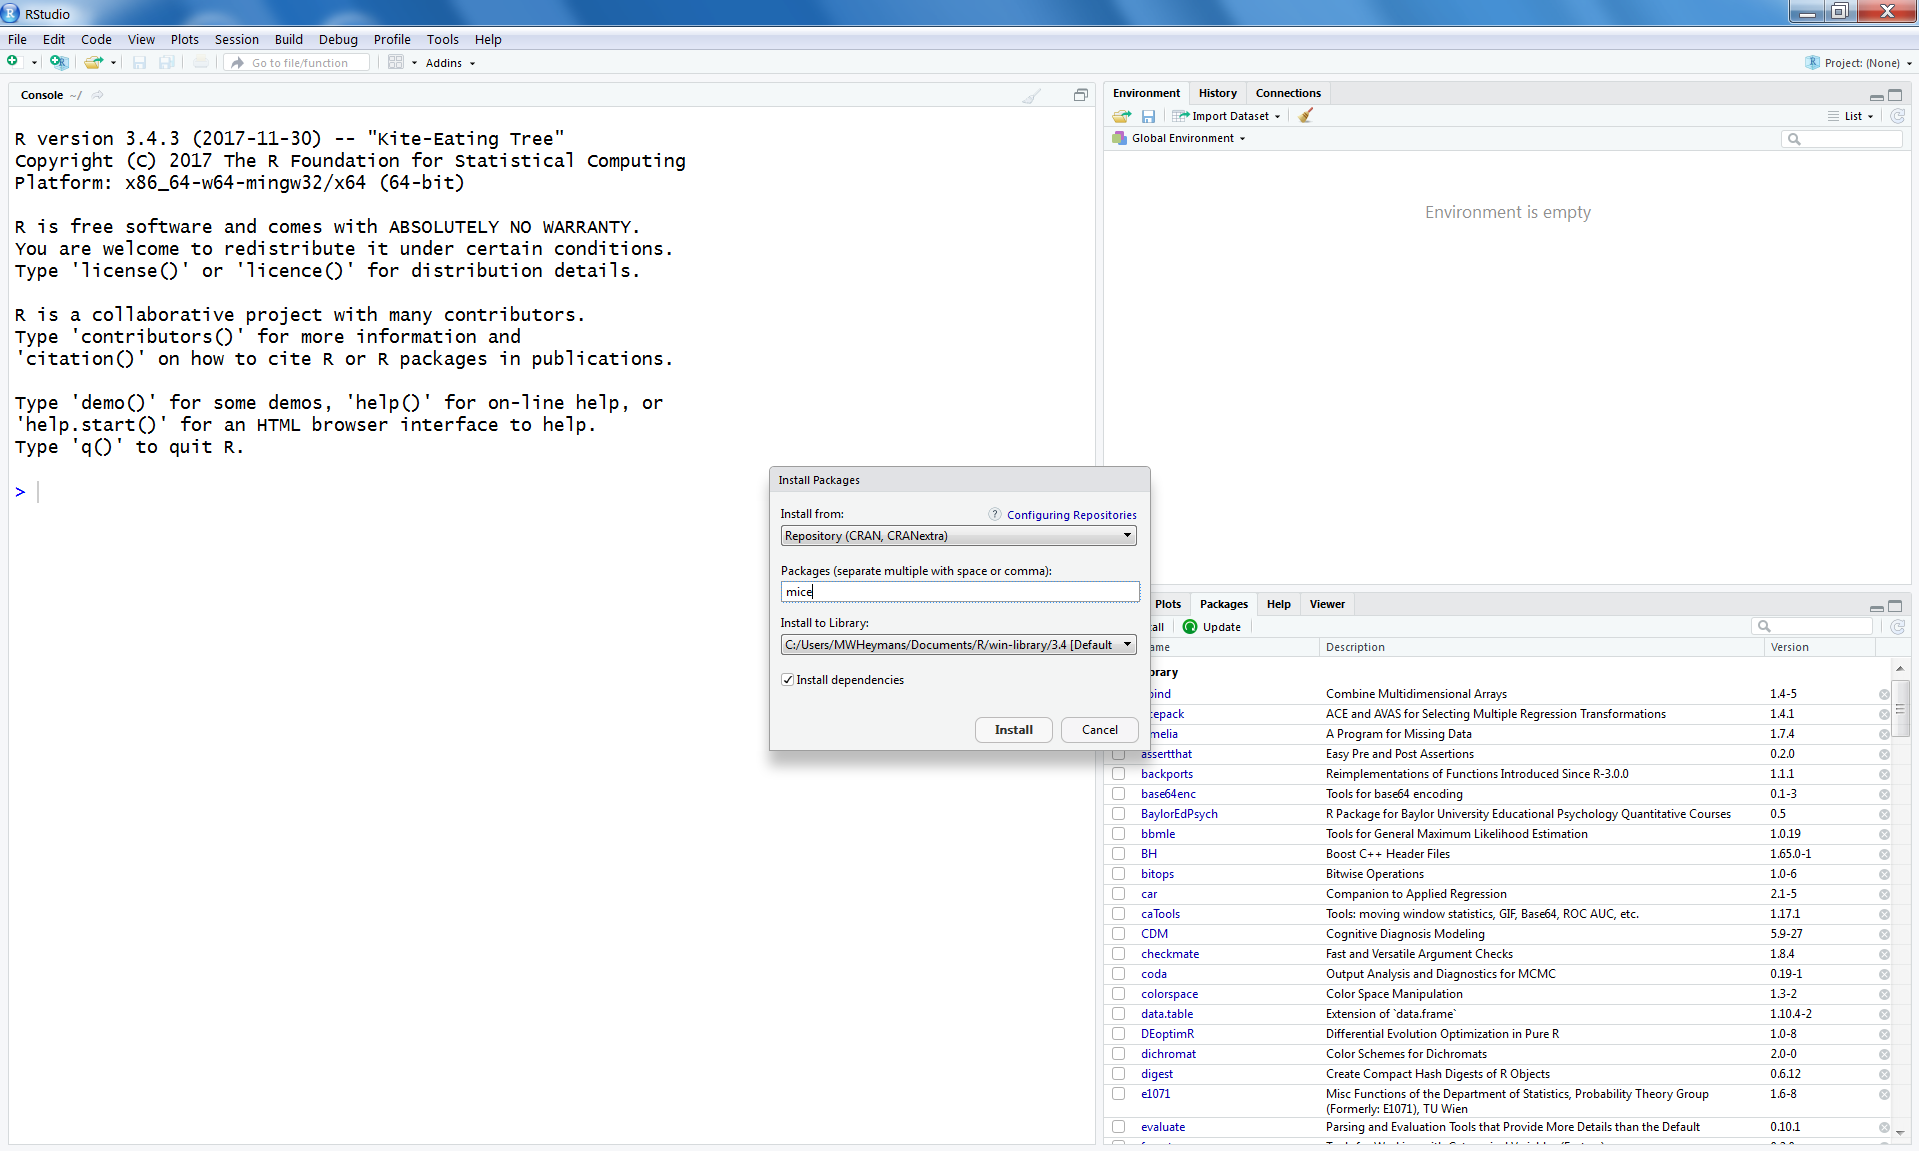
\includegraphics[width=0.9\linewidth]{images/fig1.25} 

}

\caption{Install packages Window in RStudio to install packages from the CRAN website}\label{fig:fig25}
\end{figure}

\begin{figure}

{\centering 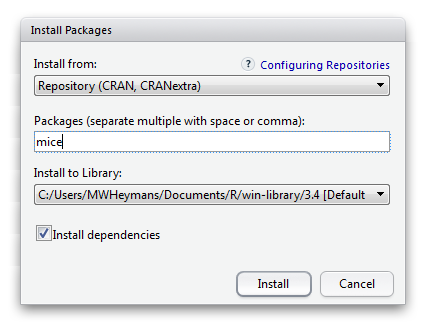
\includegraphics[width=0.9\linewidth]{images/fig1.25b} 

}

\caption{Enlarged Install packages Window in RStudio to install packages from the CRAN website}\label{fig:fig25b}
\end{figure}

\begin{figure}

{\centering 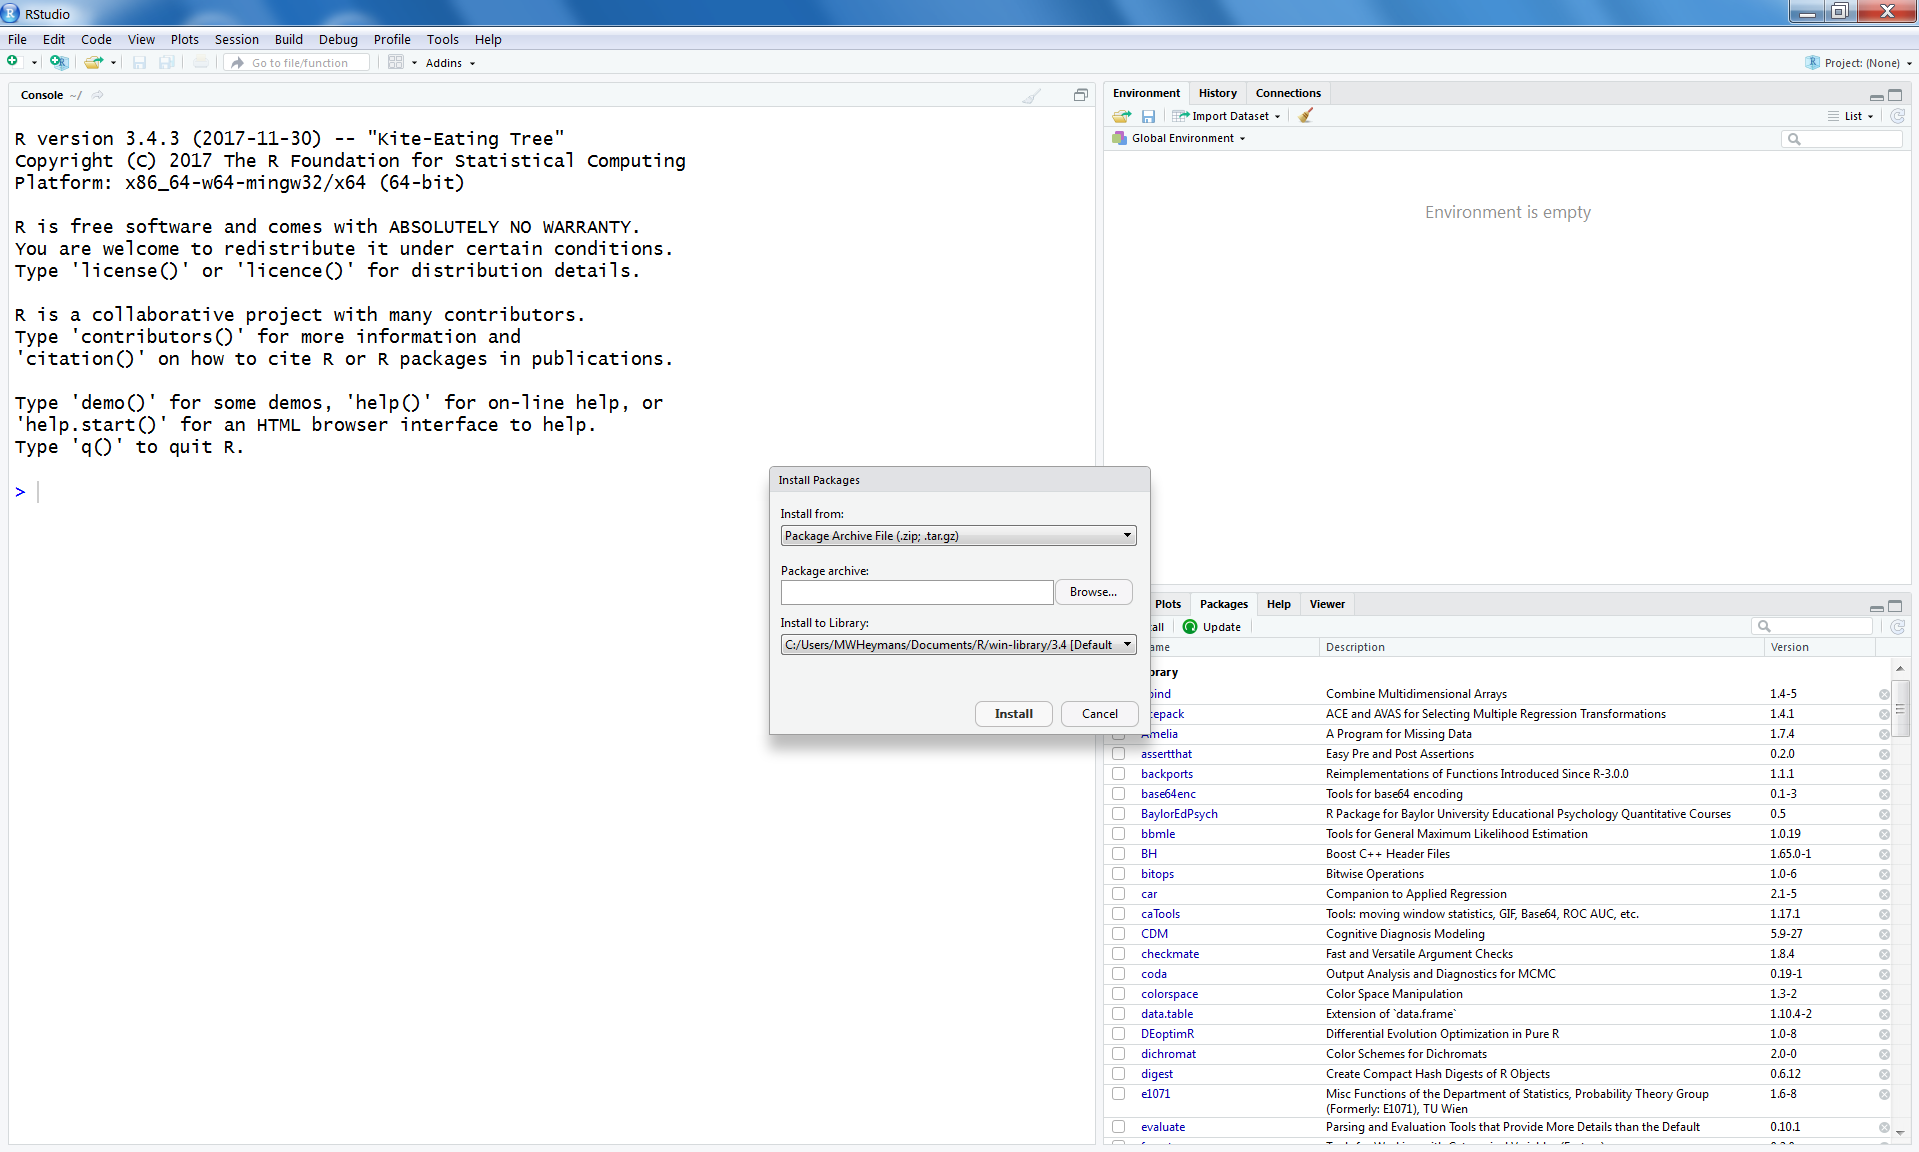
\includegraphics[width=0.9\linewidth]{images/fig1.26a} 

}

\caption{Install packages Window in RStudio to install packages from zip files}\label{fig:fig26a}
\end{figure}

\begin{figure}

{\centering 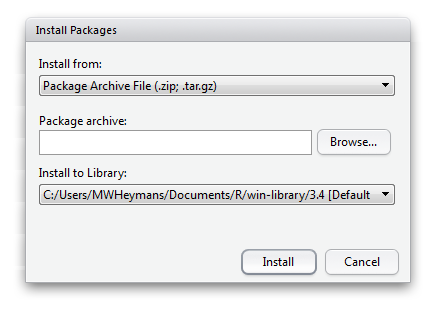
\includegraphics[width=0.9\linewidth]{images/fig1.26b} 

}

\caption{Enlarged Install packages Window in RStudio to install packages from zip files}\label{fig:fig26b}
\end{figure}

\bibliography{book.bib,packages.bib}


\end{document}
